% bachelor.tex
% Copyright 2016 Zheng Xie <xie.zheng777@gmail.com>
% https://github.com/Tedxz/xjtuthesis-x
%
% This work may be distributed and/or modified under the
% conditions of the LaTeX Project Public License, either version 1.3
% of this license or (at your option) any later version.
% The latest version of this license is in
% http://www.latex-project.org/lppl.txt
% and version 1.3 or later is part of all distributions of LaTeX
% version 2005/12/01 or later.
%
% This work has the LPPL maintenance status `maintained'.
%
% The Current Maintainer of this work is Zheng Xie.
%
% xjtuthesis-x is a Derived Work of xjtuthesis. The original maintainer of
% xjtuthesis is Weisi Dai (multiple1902 <multiple1902@gmail.com>),
% who published the project on https://code.google.com/p/xjtuthesis/ (no
% longer accessable). Currently, xjtuthesis is maintained by Aetf, and can
% be accessed on https://github.com/Aetf/xjtuthesis.
%
% xjtuthesis-x includes bug fixes, new features and a user guide.
% For detail, please refer to Readme.md.
%
% If you want to contribute to xjtuthesis-x or become the maintainer of
% xjtuthesis-x, please feel free to contact me.

\documentclass[
bachelor,
%bigskip, % sets linespread factor to 1.5
%truefont, % just turn it on when using Windows
nofont, % remember to manally set the fonts
pdflinks,
%colorlinks,
% compact,
]{xjtuthesis}

\begin{document}

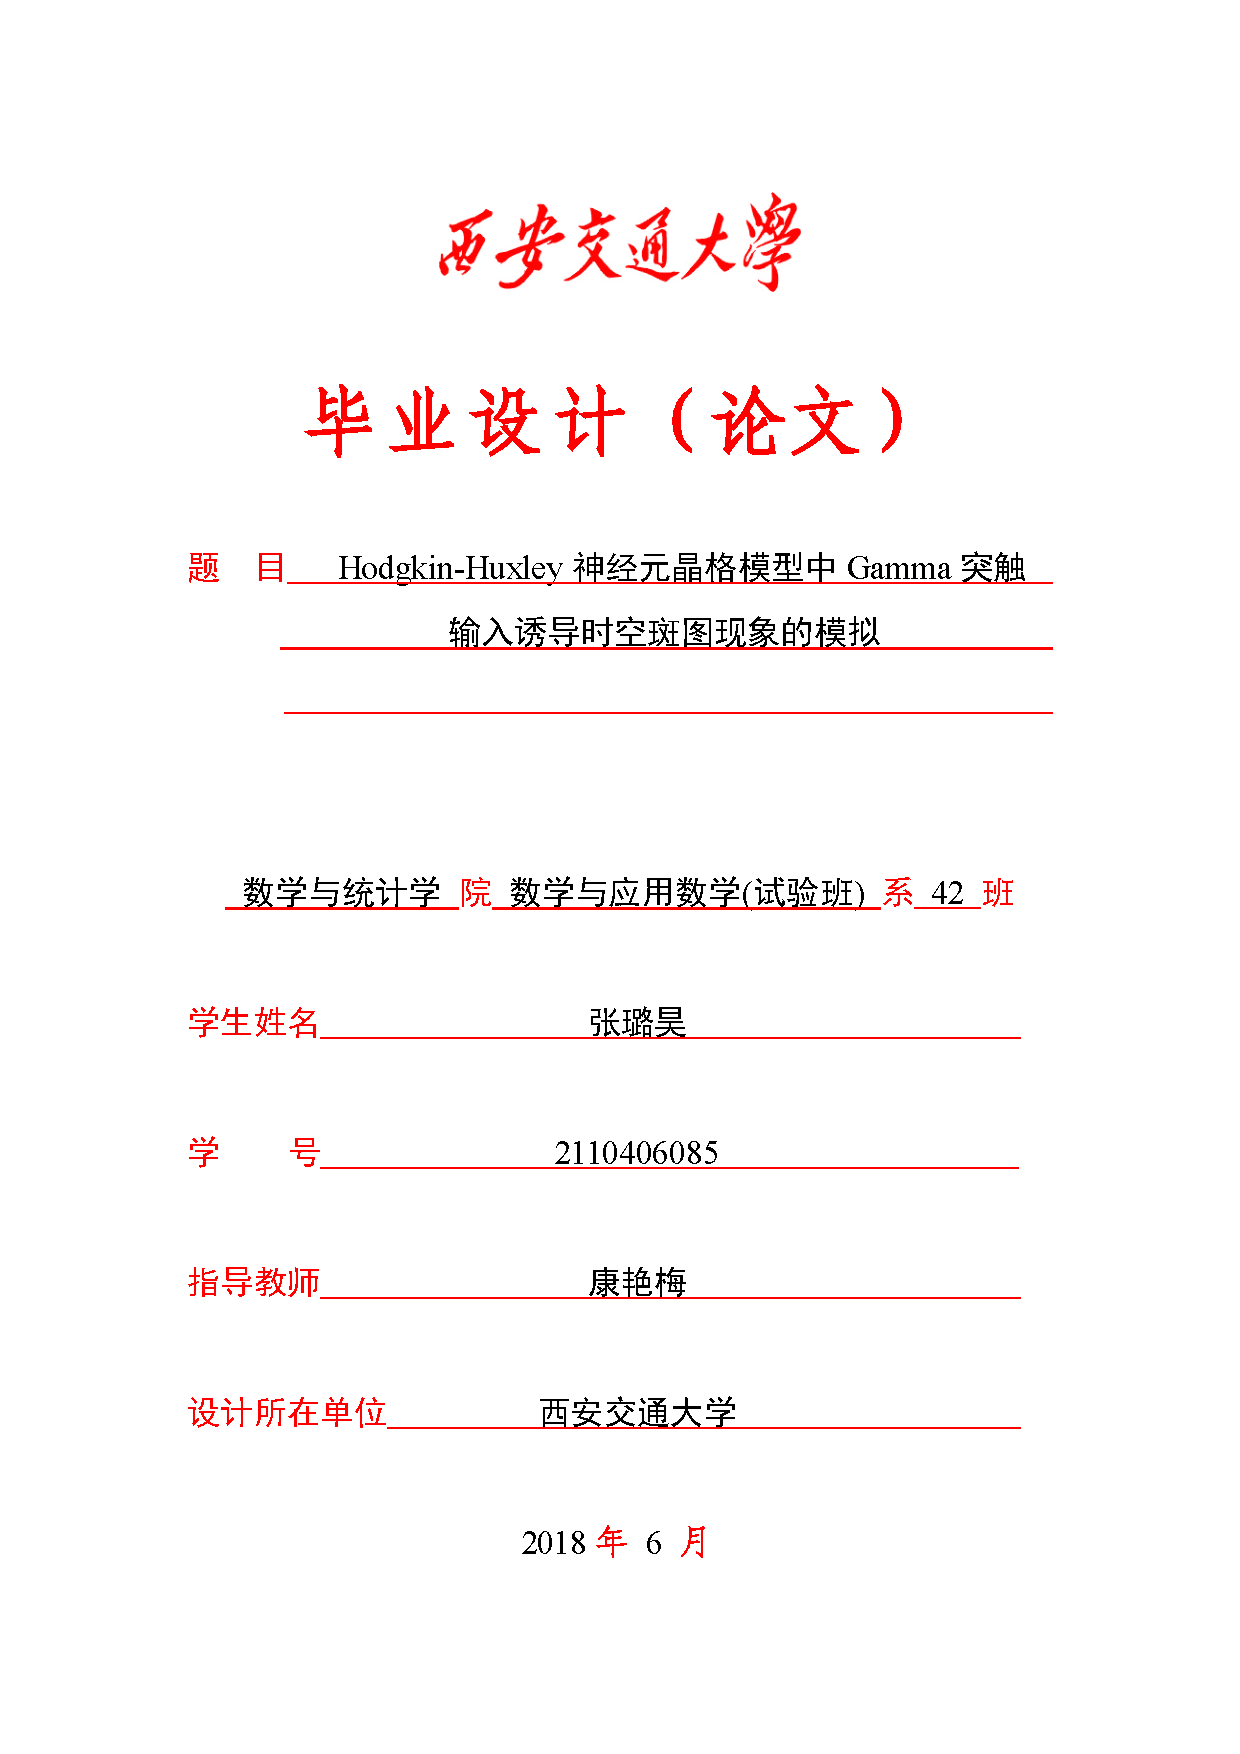
\includepdf[pages=-,scale=1,frame=false,offset=0em 4em]{extra//cover.pdf}
\pagenumbering{Roman}
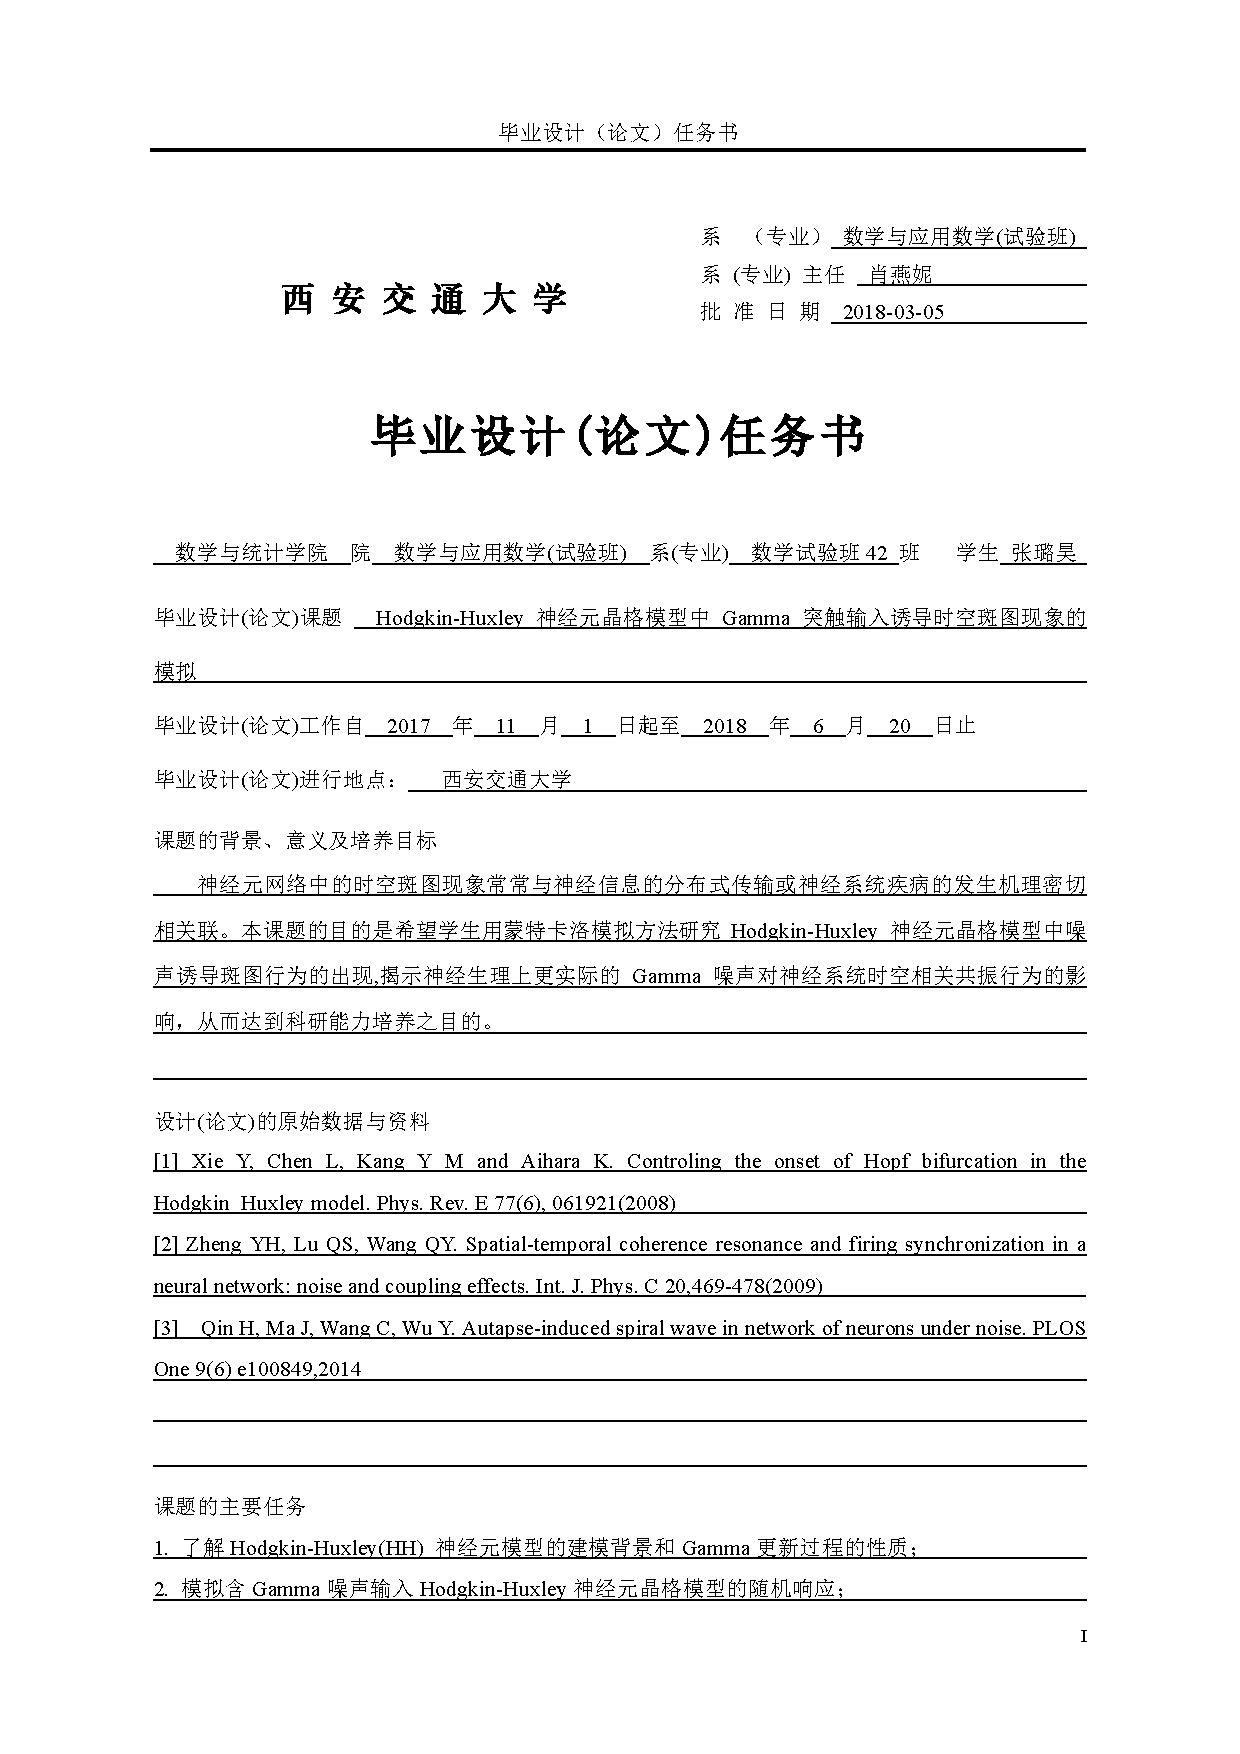
\includepdf[pages=-,scale=1,frame=false,offset=0em 4em]{extra//assignment.pdf}
% 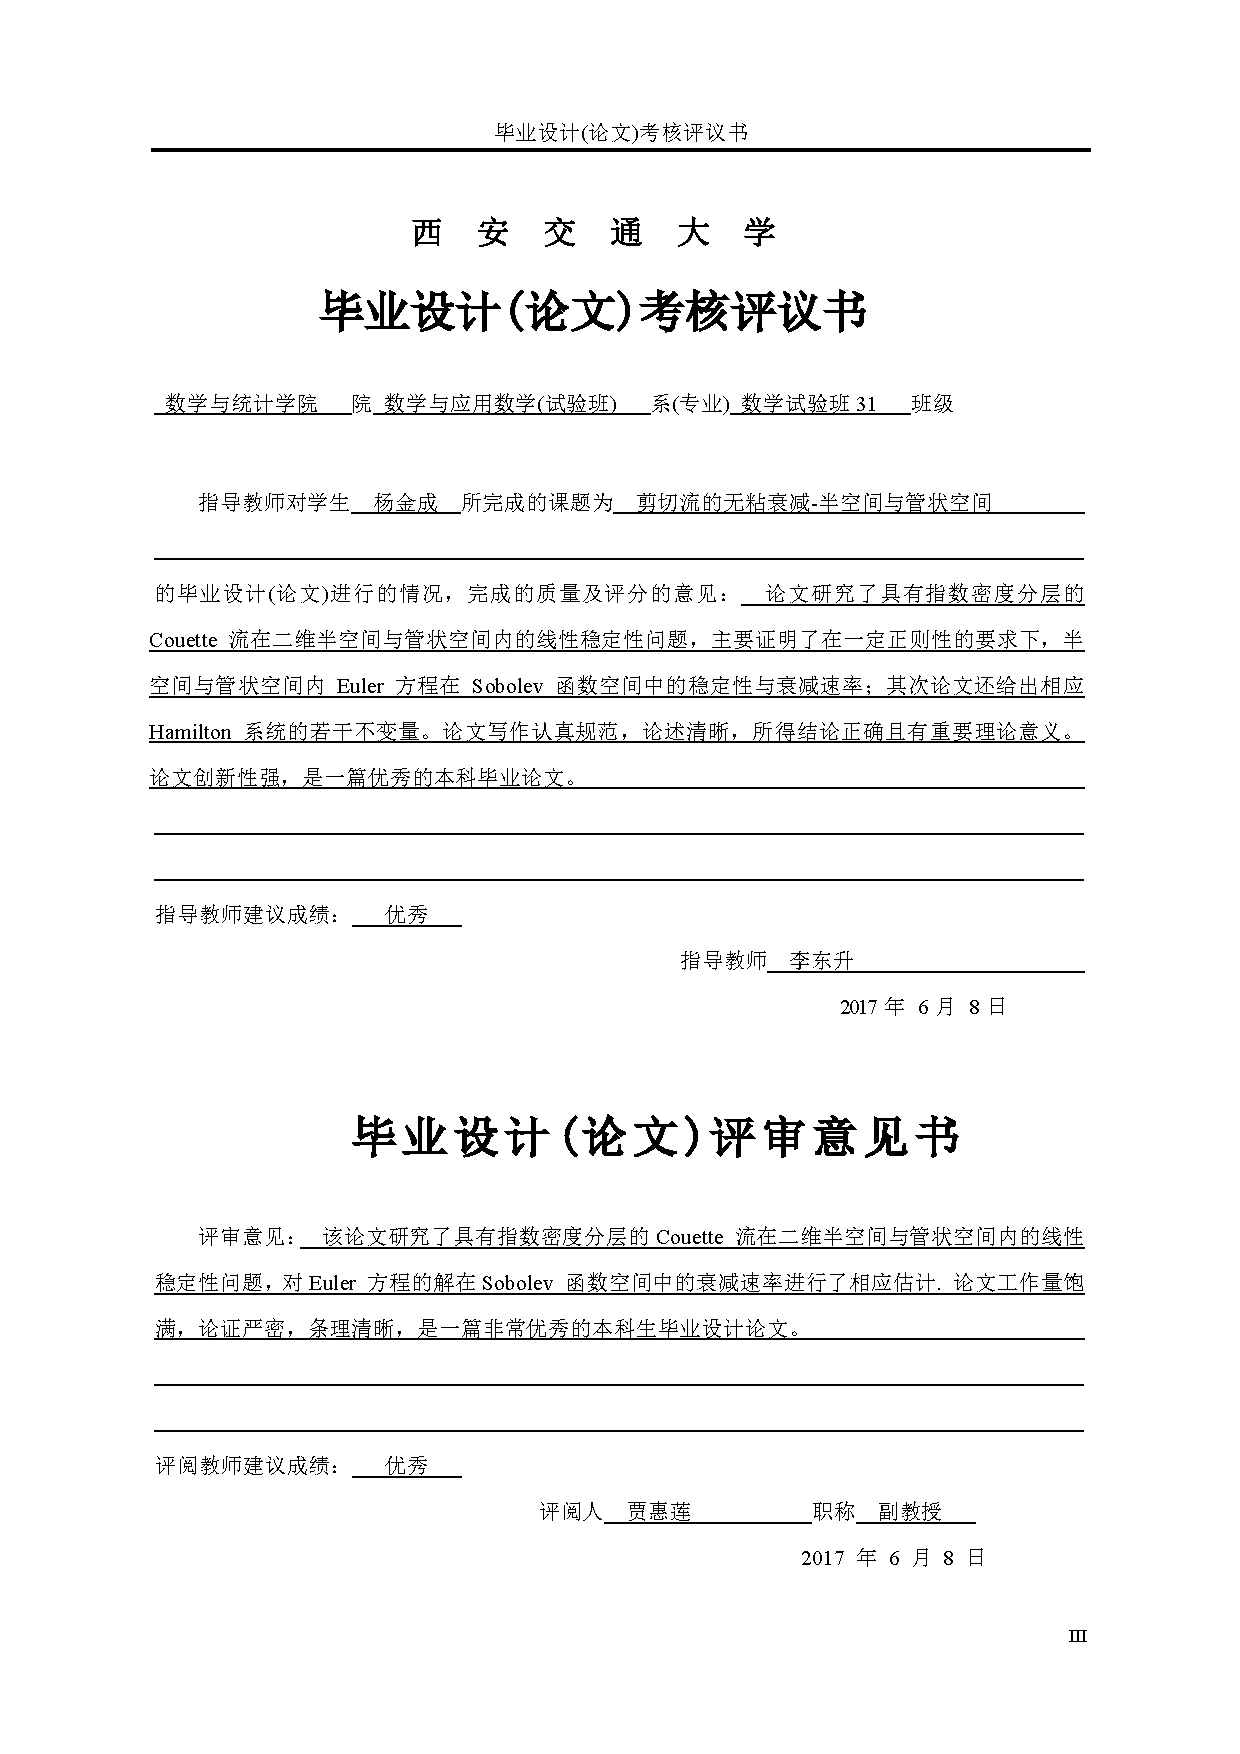
\includepdf[pages=-,scale=1,frame=false,offset=0em 4em]{extra//review.pdf}
% 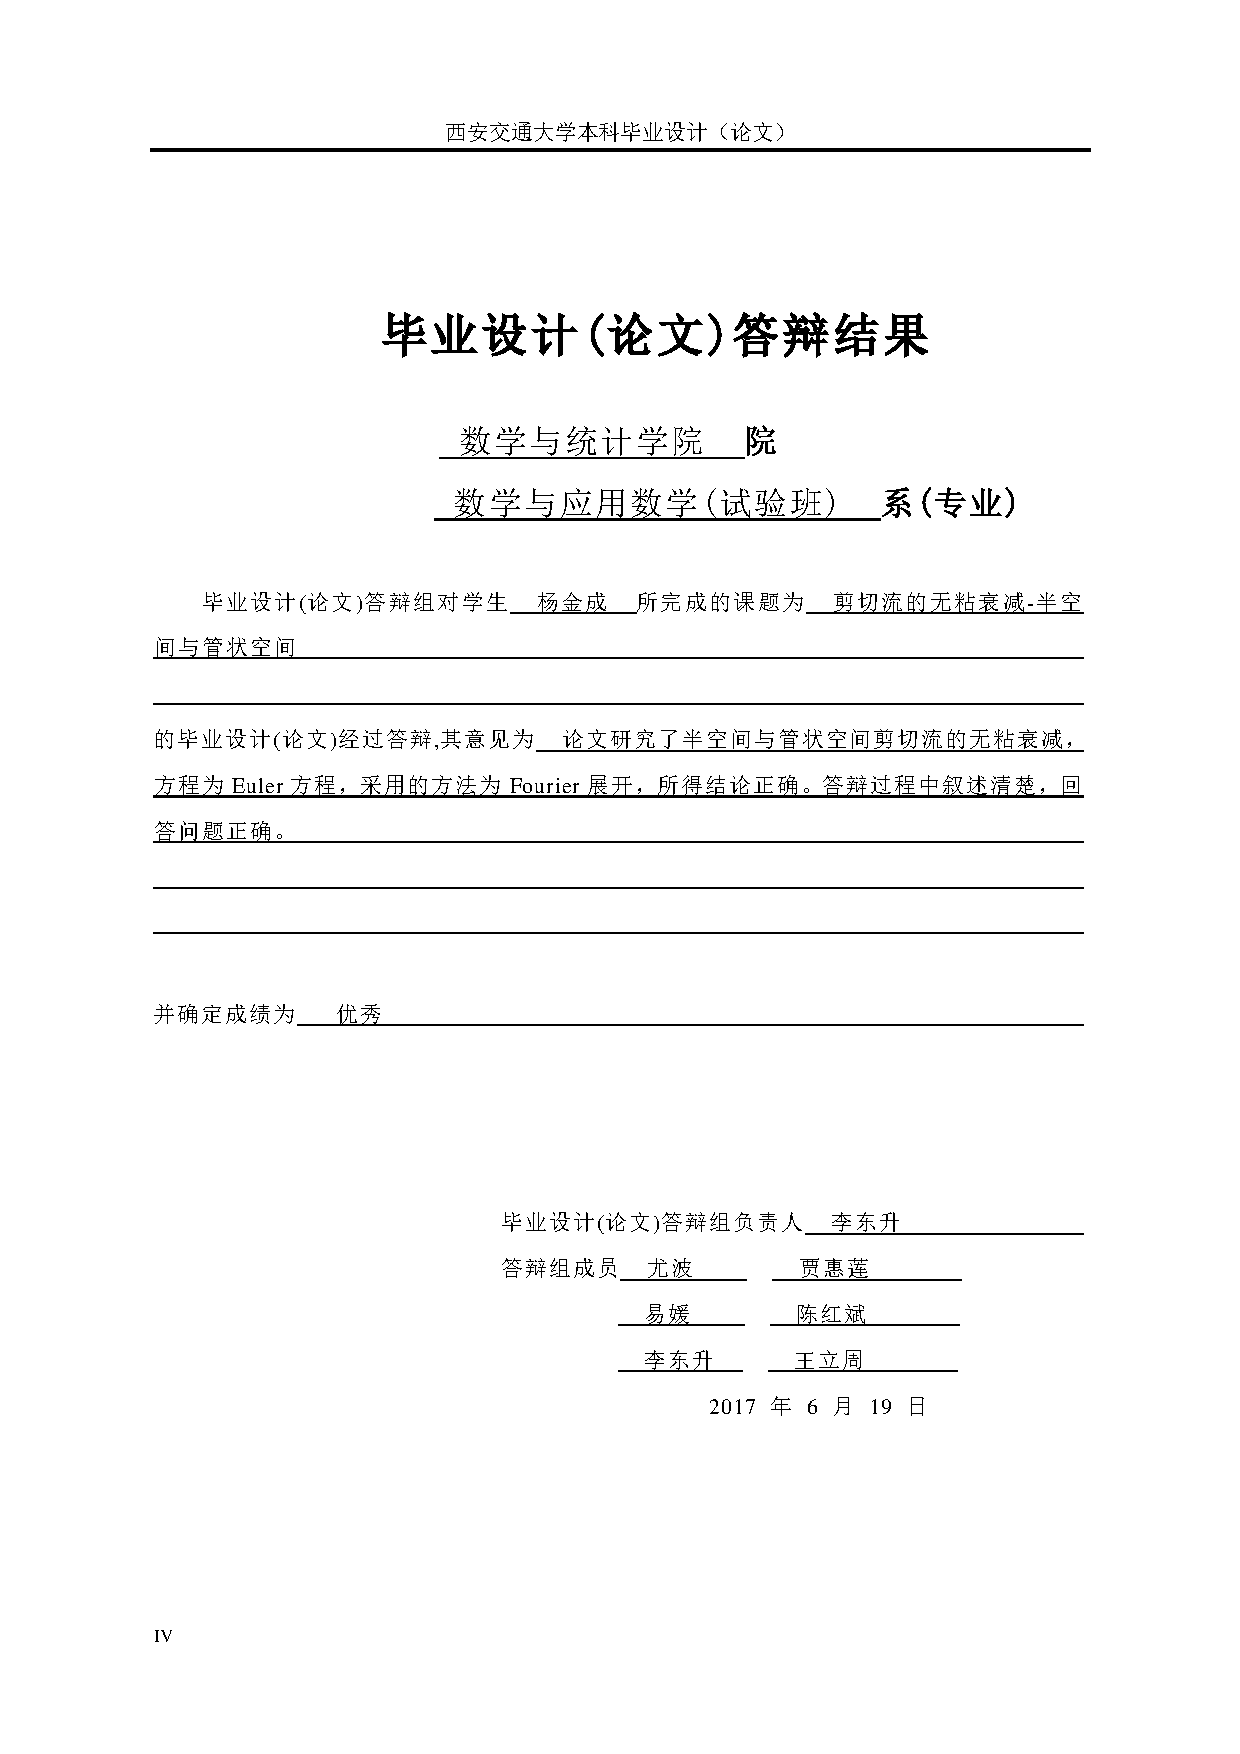
\includepdf[pages=-,scale=1,frame=false,offset=0em 4em]{extra//result.pdf}
% meta.tex
% Copyright 2016 Zheng Xie <xie.zheng777@gmail.com>
% https://github.com/Tedxz/xjtuthesis-x
%
% This work may be distributed and/or modified under the
% conditions of the LaTeX Project Public License, either version 1.3
% of this license or (at your option) any later version.
% The latest version of this license is in
%   http://www.latex-project.org/lppl.txt
% and version 1.3 or later is part of all distributions of LaTeX
% version 2005/12/01 or later.
%
% This work has the LPPL maintenance status `maintained'.
%
% The Current Maintainer of this work is Zheng Xie.
%
% xjtuthesis-x is a Derived Work of xjtuthesis. The original maintainer of
% xjtuthesis is Weisi Dai (multiple1902 <multiple1902@gmail.com>),
% who published the project on https://code.google.com/p/xjtuthesis/ (no
% longer accessable). Currently, xjtuthesis is maintained by Aetf, and can
% be accessed on https://github.com/Aetf/xjtuthesis.
%
% xjtuthesis-x includes bug fixes, new features and a user guide.
% For detail, please refer to Readme.md.
%
% If you want to contribute to xjtuthesis-x or become the maintainer of
% xjtuthesis-x, please feel free to contact me.

% 标题,中文
\ctitle{Hodgkin-Huxley神经元晶格模型中Gamma突触输入诱导时空斑图现象的模拟}

% 作者,中文
\cauthor{张璐昊}

% 学科,中文,本科生不需要
% \csubject{}

% 导师姓名,中文
\csupervisor{康艳梅}

% 关键词,中文。用全角分号「;」分割
% 研究生的应首先从《汉语主题词表》中摘选
\ckeywords{Euler方程;无粘衰减}

% 提交日期,本科生不需要
% \cproddate{\the\year 年\the\month 月}

% 论文类型,中文,本科生不需要
% 从理论研究、应用基础、应用研究、研究报告、软件开发、设计报告、案例分析、调研报告、其它中选择
% \ctype{理论研究}

% 论文标题,英文
\etitle{xxxxxxxxxxxxx}

% 作者姓名,英文
\eauthor{Luhao Zhang}

% 导师姓名,英文
\esupervisor{Yanmei Kang}

% 关键词,英文。用半角分号和一个半角空格「; 」分割
\ekeywords{Euler Equation; Inviscid Damping}

% 学科门类,英文,本科生不需要
% 从Philosophy(哲学)、Economics(经济学)、Law(法学)、Education(教育学)、Arts(文学)、
%   Science(理学)、Engineering Science(工学)、Medicine(医学)、Management Science(管理学)中选择
% \ecate{Science}


% 摘要,中文。段间空行
\cabstract{
本文研究了具有指数密度分层的Couette流在二维半空间与管状空间内的线性稳定性问题. 在全空间内, 该问题的渐近稳定性与无粘衰减速率已经得到一个比较完整的分析. 相比于全空间而言, 研究更符合物理背景的半空间内和管状空间内方程的无粘衰减的文献则较少. 本文对于证明半空间与管状空间内Euler方程在Sobolev函数空间中的稳定性与衰减速率进行了初步尝试. 针对不同情况, 我们分别得到了在一定正则性的要求下的衰减速率与稳定性. 在一定条件下, 速度场在$L^2$意义下会有水平方向$t^{-\frac{1}{2}+\nu}$, 竖直方向有$t^{-\frac{3}{2}+\nu}$的衰减速率, 或者至少在非周期方向上的投影具有这样的衰减速率. 得到的这些衰减速率与全空间中的结论一致, 尽管它提出了一些不太合理的更高的正则性要求. 对于另一些情形, 有文献证明了流函数不存在衰减. 本文对这样的特征周期解则给出了显式的构造. 之后, 本文阐明了半空间和管状空间的解有着相似的结构. 我们还研究了该Hamilton系统的若干不变量, 这为将来的研究工作带来了一些启发. 然而, 这些不变量有无穷多个负方向, 所以无法用来证明方程的非线性稳定性.
}

% 摘要,英文。段间空行
\eabstract{
We study the linear stability of an exponentially stratified Couette flow in a half space and in a finite channel. A thorough analysis of the linear asymptotic stability and inviscid damping rate had been carried out for the whole space case. Comparing to the whole space, the study about the half space or the finite channel, which suits better the physics background, are relatively inadequate. This paper makes a naive attempt to show the linear stability and inviscid decay rate of the solutions to Euler equation in the half space and in the finite channel as functions in the Sobolev space. Decay rates of the solutions with certain regularity requirements or stability are obtained under different circumstances. Under certain assumptions, the velocity field has a decay rate in $L^2$ sense of $t^{-\frac{1}{2}+\nu}$ in the horizontal direction, and $t^{-\frac{3}{2}+\nu}$ in the verticle direction, or at least the projection perpendicular to the neutral spectrum has such decay rates. These rates are basically consistent with the decay rate in the whole space, although some not quite reasonable assumptions must been applied to reach the regularity requirements. For other cases, literature has shown nonexistance of decay for the stream function. We give explicit construction of such periodic eigensolutions. Afterwards, similar structure of the solutions in a half space and in a finite channel are compared. We also studied the Hamiltonian structure and invariants of the system, which brought some inspiration for the study. Unfortunately, all these invariants have infinitely many negative direction, hence they are unable to make any contribution for the proof of nonlinear stability.
}


% 致谢
\acknowledgement{
本文是在西安交通大学的李东升老师与佐治亚理工学院的林治武老师的共同指导下完成的, 受到美国国家科学基金会NSF (grantDMS-1411803)项目的资助. 林治武老师为论文的选题, 文献资料的选择提供了十分有益的指导, 并十分关照本人的工作进展, 使得论文得以顺利完成. 在佐治亚理工学院实习期间, 林治武老师组织的丰富的讨论班与讲座也给予了我很多启发. 同时也需要在此感谢学校拔尖办给予我此次出访机会, 感谢佐治亚理工学院的同僚们的帮助, 让我能够进行这样一项很有意义的科研. 另外, 本毕业设计虽然是在外校完成的, 李东升老师仍然给予了相当细致的关照与充分的支持, 本文的完成离不开他的帮助. 谨向林治武老师与李东升老师致以衷心的感谢! 
} % 请修改 meta.tex 中的论文元信息 
\xjtucinfopage
\xjtueinfopage
\xjtutoc
\clearpage
% \input{pages/denotation.tex} % 主要符号表,可以没有

\xjtucontent


\chapter{绪论}

康老师的研究\cite{xie2008change}很厉害!

\section{课题背景及意义}
神经元网络中的时空斑图现象常常与神经信息的分布式传输或神经系统疾病的发生机理密切相关联。

\medskip
由于生物对象的极端复杂性,生物系统普遍具有多变量、非线性、强耦合的特点。经典Hodgkin-Huxley模型即为利用微分方程组描述神经元细胞跨膜电压与离子电流变化的复杂非线性系统,因此若对其进行数学分析,传统的线性
理论已不适用,必须采用非线性系统理论对生物模型进行动态分析。在非线性理论中,分岔理论就是很重要的一种理论。
\medskip
分岔理论反映了流的拓扑结构随参数的变化而引起质的变异,不论在数学理论上还
是在现实应用中都具有极为重要的意义。


噪声在许多非线性动力系统中有着建设性的作用。相关文献已经证明了适量的噪声可以对弱信号进行共振放大,
这就是所谓的随机共振〔1—3〕。特别地,噪声
即使在缺乏弱确定性的情况下也能起到排序作用。
刺激,由此建立的术语描述现象。
是相干共振〔4—7〕。特别是在生化反应中
在某种程度上,这是一个相当坚定的事实。
随机性是不可避免的。因此,许多研究已经
用于各种生物过程,其中
研究了噪声的建设作用。它已经被
示出,噪声可以引起随机钙振荡
亚阈值系统,从而获得最佳的时间顺序
通过中等强度的噪声〔8—11〕。类似的研究也有
也进行了昼夜节律[12,13]以及
遗传调节〔14〕和神经元系统[15,16]。
值得注意的是,噪声引起的共振现象不是。
仅限于时间动态的调整。几个
研究也集中在空间或时空上。
生物化学介质的动力学〔17—19〕
研究了噪声对时空有序性的影响。
已经发现,单独使用噪声通常足以诱导。
不同系统中的时空有序行为
光学器件和生化介质[20,21]。特别地,
首次报道了时空随机共振。
〔22〕用于可兴奋系统。此外,还存在研究。
噪声引起的螺旋生长和增强
时空顺序〔23—25〕,噪声持续相干性
时空簇与自组织临界性〔26〕噪声
诱导兴奋性〔27〕,噪声诱导传播
谐波信号〔28〕以及噪声的持续和控制
空间扩展系统中的同步〔29〕。
最近,特别是噪声引起的空间动力学。
空间扩展系统中的兴奋事件
详细调查。卡里略等人。〔30〕已表明:
对于非线性介质,在形成不稳定图形的情况下,有
存在一个加性时空噪声的中间值
圆平均空间结构函数的峰值
最好解决,从而标记空间相干共振
系统。近年来,这一概念得到了扩展和空间相干性。
可激发介质中的共振现象
[31,32]和具有不同拓扑结构的网络〔33〕。

\section{相干共振}

\section{螺旋波}

\section{Hodgkin-Huxley模型}

\newcommand{\ai}{\alpha_i}
\newcommand{\am}{\alpha_m}
\newcommand{\an}{\alpha_n}
\newcommand{\ah}{\alpha_h}

\newcommand{\ambar}{\overline{\am}}
\newcommand{\anbar}{\overline{\an}}
\newcommand{\ahbar}{\overline{\an}}

\newcommand{\bi}{\beta_i}
\newcommand{\bm}{\beta_m}
\newcommand{\bn}{\beta_n}
\newcommand{\bh}{\beta_h}

\newcommand{\bmbar}{\overline{\bm}}
\newcommand{\bnbar}{\overline{\bn}}
\newcommand{\bhbar}{\overline{\bn}}

\newcommand{\go}{G_{\omega}}
\newcommand{\gna}{G_{Na}}
\newcommand{\gk}{G_{K}}
\newcommand{\gl}{G_{l}}

\newcommand{\gobar}{\overline{g_{\omega}}}
\newcommand{\gnabar}{\overline{g_{Na}}}
\newcommand{\gkbar}{\overline{g_{K}}}
\newcommand{\glbar}{\overline{g_l}}

\newcommand{\vna}{V_{Na}}
\newcommand{\vk}{V_{K}}
\newcommand{\vl}{V_{l}}

\newcommand{\vmbar}{\overline{V_m}}
\newcommand{\vnbar}{\overline{V_n}}
\newcommand{\vhbar}{\overline{V_h}}

Hodgkin-Huxley模型直接反映了细胞膜上离子通道的开闭情况。细胞膜内外电流的流入流出可以简化为一个电容和电阻并联的模型,如下图所示\cite{gerstner2002spiking}:
\begin{figure}[!ht]
\centering
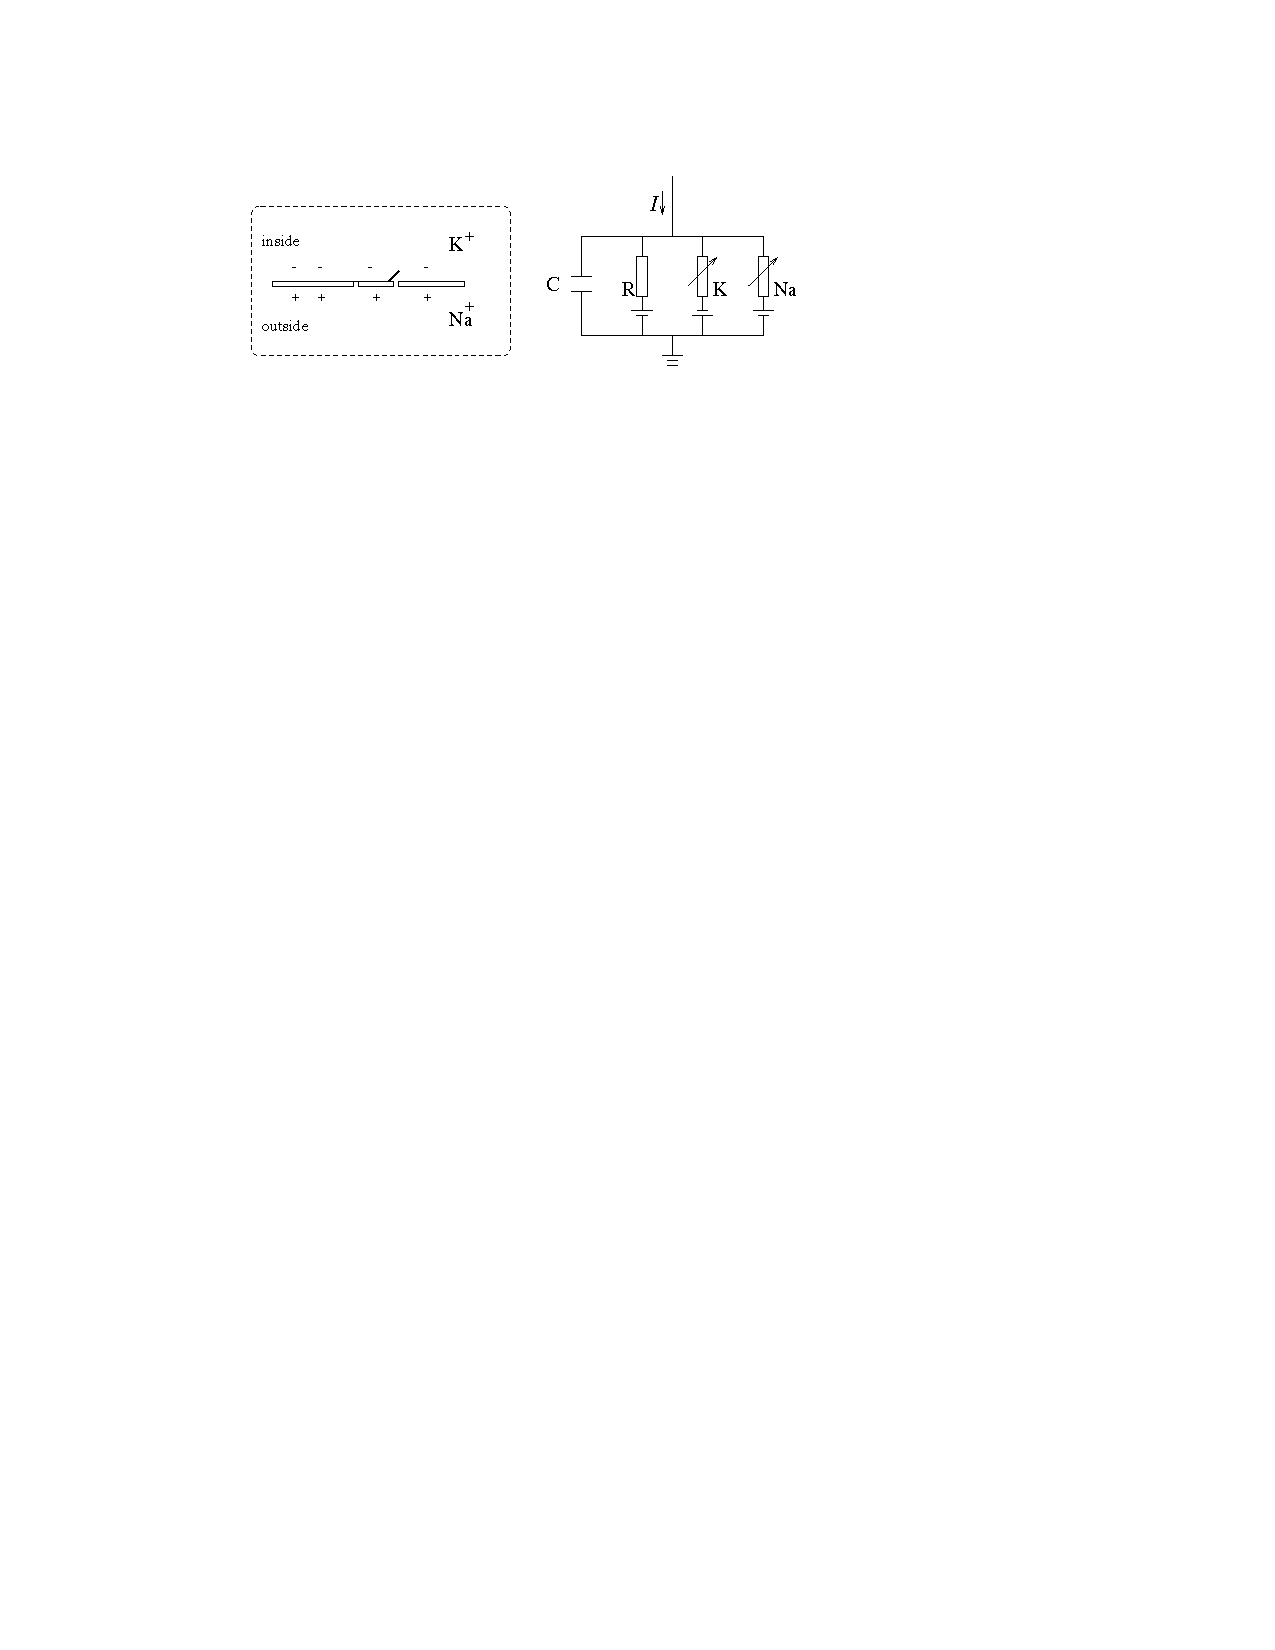
\includegraphics[scale=1]{moxingjiantu.pdf}
\caption{Hodgkin–Huxley模型的简图}
\end{figure}\\
在此等效电路中,跨膜流动的电流可以分为两个部分:一部分与膜电容的充电有关;另一部分涉及到不同类型的离子的跨膜流动。离子电流可以进一步分为三部分:钠离子电流$I_{Na}$,钾离子电流$I_K$,和很小的主要由氯离子引起的漏电流$I_l$。

\medskip
根据基尔霍夫电流定律,取电路上一个节点,根据任意时刻流入节点的电流之和等于流出节点的电流之和,在这个问题上即为,外部电流$I(t)$通过各个离子通道进出细胞膜电流$I_{k}(t)$,或者直接留在细胞膜两侧,成为细胞膜这个电容上的电荷,也就是对这个电容充放电的电流$I_{cap}(t)$,可以列出以下方程:
\begin{align}
I(t)=I_{cap}(t)+\sum_k I_{k}(t)
\end{align}
把电容的充放电显式表示出来,也就是用$C_m\dfr{v}{t}$替代$I_{cap}(t)$,我们可以得到
\begin{align}
C_m \dfr{v}{t}=-\dfrac{V-V_{eq}}{R}+\sum_k I_{k}(t)
\end{align}
其中$C_m$是单位面积上的膜电容量,$R$是膜电阻,$V$是此时的膜内外电位差(即膜电位),$V_{eq}$是细胞膜的静息电位,两者之差$V-V_{eq}$是促使膜两边带电离子运动的主要动力。

考虑到生物细胞膜上的各种离子通道的不同作用效果,后续的模型依据神经细胞的生理基础上建立了许多相应的各种生物物理模型,他们建立的模型中涉及到较多的不同离子通道的电导率和各通道打开的概率的参数。例如Hodgkin 和Huxley考虑了钠离子通道和钾离子通道作为膜电阻的主要来源,认为离子驱动力是膜电位及其平衡电位之差,将驱动力乘以某一适当的电导率就可得到相应的离子电流,即式子中的$k$有三种枚举值,即图1右图所示。为了解释实验数据,Hodgkin和Huxley猜测$\gna$和$\gk$(即K和Na的离子通道的宏观电导)随膜电势动态变化。今天我们已经知道这一电压依赖性的是与离子通道的生理性质相关的,但是为了方便起见,我们这里依然沿用Hodgkin和Huxley的观点。 Hodgkin-Huxley模型中的宏观电导$\gk$可以被看作是大量微观离子通道的集体效应,每个离子通道可以被看作是含有几个可以控制离子流动的“门”。每个门只能处于开放或者关闭这两个状态。当某一离子通道的所有门都处于开放状态时,这个离子通道才是打开的。否则,如果任意一个门是处于关闭状态的,则这个离子通道是关闭的。Hodgkin和Huxley假设,每个门处于开放或者关闭的概率是依赖于膜电压的。考虑一个特定的门$i$,定义0到1之间的概率$p_i$为单个门处于开放状态的概率。如果离子通道数非常大,则可以将$p_i$认为是处于开放状态的门的数目与总的门数目之比,而将$1-p_i$认为是处于关闭状态的门的数目与总的门数目之比。在HH模型中,开放与关闭状态间的转变服从一阶的动力学把上述方程改写成以下形式:
\begin{align}
\dfr{p_i}{t}= \ai (V)(1-p_i)-\bi (V)p_i
\end{align}
当一个单独的通道打开时(即当所有的门打开时),它才对宏观电导有贡献。因此,一群离子通道的宏观电导正比于处于开放状态的通道数目,亦即正比于处于门开放状态的概率。含有$\omega$种门的离子通道的宏观电导正比于门的概率$p_i$的乘积:
\begin{align}
\go = \gobar \prod_i p_i
\end{align}
这里,$\gobar$是归一化的常数,是所有离子通道打开时的最大电导。在HH模型中,钠电导用3个$m$门和1个$h$门来模拟,钾电导用4个$n$门来模拟,即
\begin{align}
\gna &= \gnabar p_m^3p_h:= \gnabar m^3h\\
\gk &= \gkbar p_n^4:= \gkbar n^4
\end{align}
由此,我们得出单个神经元的Hodgkin-Huxley 模型的标准形式如下:
\begin{align}
\notag \dfr{V}{t} &= - \dfrac{1}{C_m} \left[ \gnabar m^3h(V-\vna)+ \gkbar n^4(V-\vk)+\glbar(V-\vl) - I \right] \\
\dfr{m}{t} &= \am (V)(1-m)-\bm (V)m \\
\notag \dfr{h}{t} &= \ah (V)(1-h)-\bh (V)h \\
\notag \dfr{n}{t} &= \an (V)(1-n)-\bn (V)n 
\end{align}
其中下标$K,Na,l$分别代表的是钾离子通道,钠离子通道,以及其他离子通道的情况,而$\gnabar m^3h,\gkbar n^4, \glbar$则分别对应他们的电导率,$\vna, \vk, \vl$则分别对应它们的平衡电位;变量$m,h,n$是假设遵从以上形式的一阶动力系统的电压依赖性门控变量(可以理解为在给定电压下相对应的这三种离子通道的开闭动态过程,因此它们的取值均在$(0,1)$之间)。









\chapter{Hodgkin-Huxley 模型的单参数Hopf分岔分析}

Hodgkin-Huxley模型一个重要的特点,是它在奇点附近随着外部电流的变化会产生Hopf分支现象。简单来说,一个非线性系统出现Hopf分支意味着系统的奇点会随着某个参数正则的变化而演化为极限环,或者由极限环退化为奇点。作为医学上最常见的细胞学模型,对系统Hopf分支的控制对于研究疾病的产生与预防有着十分大的作用。研究表明如奥茨海默症、帕金森病、焦虑、注意力不足过动症(ADHD)和思觉失调症等等都可能与非线性控制系统的Hopf分支有关。

\medskip

我们考虑二维空间$\Omega=(0,\pi) \times (0,\pi)$下满足Neumann边值条件的Hodgkin-Huxley神经元规则网络动力学方程为:
\begin{align}
\notag \pfr{V}{t} &= -\dfrac{1}{C_m} \left[ \gnabar m^3h(V-\vna)+ \gkbar n^4(V-\vk)+\glbar(V-\vl) -D \Delta V -I \right] \\
\pfr{m}{t} &= \am (V)(1-m)-\bm (V)m \\
\notag \pfr{h}{t} &= \ah (V)(1-h)-\bh (V)h \\
\notag \pfr{n}{t} &= \an (V)(1-n)-\bn (V)n 
\end{align}
其中$\ai (V), \bi (V)$分别为跨膜电压V的函数,采取如下形式:
\begin{align}
\notag \am &= \dfrac{\ambar (V-\vmbar)}{1- e^{-(V-\vmbar)/K_{\am}}} \\
\notag \bm &= \bmbar e^{-(V-\vmbar)/K_{\bm}}\\
\notag \ah &= \ahbar e^{-(V-\vhbar)/K_{\ah}}\\
\bh &= \dfrac{\bhbar }{1- e^{-(V-\vhbar)/K_{\bh}}} \\
\notag \an &= \dfrac{\anbar (V-\vnbar)}{1- e^{-(V-\vnbar)/K_{\an}}} \\
\notag \bn &= \bnbar e^{-(V-\vnbar)/K_{\bn}}
\end{align}
并记$X=(V,m,n,h)^T$。

\section{HH模型的平衡点与稳定性}
根据生理意义,HH模型描述的系统首先在细胞静息状态应当有平衡点$X_0=(V_0,m_0,h_0,n_0)^T$,其中$V_0$代表细胞膜静息电位。若变量$V,m,h,n$偏离平衡状态,经过一段时间后仍将回到平衡值。则其平衡点满足以下条件:
\begin{align}
\notag & -\gnabar m^3h(V_0 -\vna)+ \gkbar n^4(V_0-\vk)+\glbar(V_0-\vl) +D \Delta V=0 \\
& m_0 = \dfrac{\am (V_0)}{\am (V_0)+\bm (V_0)} \\
\notag & h_0 =\frac{ \ah (V_0)}{ \ah (V_0)+ \bh (V_0)} \\
\notag & n_0= \frac{\an (V_0)}{\an (V_0)+\bn (V_0)}
\end{align}
为计算方便,将系统写成如下形式:
\begin{align}
\notag \pfr{V}{t} &= f_V(V,m,h,n)+D\Delta V\\
\pfr{m}{t} &= f_m(V,m) \\
\notag \pfr{h}{t} &= f_h(V,h)\\
\notag \pfr{n}{t} &= f_n(V,n) 
\end{align}
在平衡点$x_0(V_{0},m_{0},h_{0},n_{0})$处对系统进行线性化,得到如下近似线性系统
\begin{align}
\notag \pfr{V}{t} &= J_{V}(V_0,m_0,n_0,h_0)\cdot
\left(
\begin{array}{c}
V-V_0\\
m-m_0\\
h-h_0\\
n-n_0
\end{array}
\right)
+D\Delta V\\
\pfr{m}{t} &= J_{m}(V_0,m_0,n_0,h_0)\cdot
\left(\begin{array}{c}
V-V_0\\
m-m_0\\
h-h_0\\
n-n_0
\end{array}
\right) \\
\notag \pfr{h}{t} &= J_{h}(V_0,m_0,n_0,h_0)\cdot
\left(
\begin{array}{c}
V-V_0\\
m-m_0\\
h-h_0\\
n-n_0
\end{array}
\right)\\
\notag \pfr{n}{t} &= J_{n}(V_0,m_0,n_0,h_0)\cdot
\left(
\begin{array}{c}
V-V_0\\
m-m_0\\
h-h_0\\
n-n_0
\end{array}
\right)
\end{align}

其中,
\begin{align}
\left(
\begin{array}{c}
J_V\\
J_m\\
J_h\\
J_n
\end{array}
\right)_{X_0}=
\left(
\begin{matrix} 
\pfr{f_V}{V} & \pfr{f_V}{m} & \pfr{f_V}{h} & \pfr{f_V}{n}\\ 
\pfr{f_m}{V} & \pfr{f_m}{m} & 0 & 0\\ 
\pfr{f_h}{V} & 0 & \pfr{f_h}{h} & 0 \\
\pfr{f_n}{V} & 0 & 0 & \pfr{f_n}{n}
\end{matrix}
\right) _{X_0}
\end{align}
定义二阶可导且满足Neumann边值条件的函数集合:
\begin{align*}
\widetilde{D_{A_1}} = \left\{ \phi\in C^2(\bar{\Omega}):
\pfr{}{x} \phi(0,y) = \pfr{}{x} \phi(\pi,y) =
\pfr{}{y} \phi(x,0) = \pfr{}{y} \phi(x,\pi) = 0 \right\},
\end{align*}
并定义$D_{A_1}$为$\widetilde{D_{A_1}}$在Sobolev空间$H^2(\Omega)$的闭包,考虑空间$D_A=D_{A_1}\times L^2(\Omega) \times L^2(\Omega) \times L^2(\Omega)$,其中$A_1$是Laplace算子$\Delta$在$D_{A_1}$上的延拓,定义$D_{A_1^2}=\{u \in D_{A_1}:A _1 u\in D_{A_1}\}$,令
\begin{align*}
\tilde{A_1}:D_{A_1^2} \rightarrow D_{A_1}
\end{align*}
为$A_1$在$D_{A_1^2}$上的限制。令
\begin{align*}
\tilde{A}=\left(
\begin{array}{cccc}
\tilde{A_1} &0 & 0 &0\\
0&0 & 0 &0\\
0 &0 & 0 &0\\
0 &0 & 0 &0
\end{array}
\right),
\end{align*}
根据参考文献\cite{hassard1981theory}上的结论,$\tilde{A}$生成$D_A$上的一个紧解析半群。令
\begin{align*}
L=DA+\left(
\begin{array}{c}
J_V\\
J_m\\
J_h\\
J_n
\end{array}
\right)_{X_0}
\end{align*}
为系统对应的稳态方程在平衡点附近的线性化算子,则$L$也生成一个紧解析半群。考虑系统的高阶项扰动$f$,则系统
\begin{align}
\dfr{X}{t}=D\tilde{A}X + \left(
\begin{array}{c}
J_V\\
J_m\\
J_h\\
J_n
\end{array}
\right)_{X_0} (X - X _0) +f(X)
\end{align}
生成局部半流。所以根据中心流形定理,当$L$恰好只有一对共轭的纯虚数特征值$\lambda$与$\bar{\lambda}$,且$L$的谱的其余部分的实部均小于一个负常数$\delta$,此时系统出现Hopf分岔。为了研究$L$的谱,我们可以考虑对系统变量进行以下余弦级数展开:
\begin{align}
\notag V(t;x,y)& =\sum_{k,j} V_{kj}(t)\cos kx \cos jy + V_0\\
m(t;x,y)& =\sum_{k,j} m_{kj}(t)\cos kx \cos jy +m_0\\
\notag h(t;x,y)& =\sum_{k,j} h_{kj}(t)\cos kx \cos jy +h_0\\
\notag n(t;x,y)& =\sum_{k,j} n_{kj}(t)\cos kx \cos jy +n_0
\end{align}
并得到:
\begin{align}
\dfrac{\partial V}{\partial t} &= \sum_{k,j} V'_{kj}(t)\cos kx \cos jy \\
\Delta V &= \sum_{k,j} (-k^2-j^2) V_{kj}(t)\cos kx \cos jy 
\end{align}
则对于线性化方程有:
\begin{align}
\notag &\sum_{k,j} V'_{kj}(t)\cos kx \cos jy = \sum_{k,j} J_{V}(V_0,m_0,h_0,n_0)
\left(
\begin{array}{c}
V_{kj}\\
m_{kj}\\
h_{kj}\\
n_{kj}
\end{array}
\right)\\
& \quad \quad \quad \quad \quad \quad \quad \quad \quad \quad \quad +D\sum_{k,j} (-k^2-j^2) V_{kj}(t)\cos kx \cos jy\\
\notag \Rightarrow & \sum_{k,j} (V'_{kj}(t)-J_{V}(V_0,m_0,h_0,n_0)
\left(
\begin{array}{c}
V_{kj}\\
m_{kj}\\
h_{kj}\\
n_{kj}
\end{array}
\right) -D(-k^2-j^2) V_{kj}(t))\cos kx \cos jy=0 \\
\Rightarrow & \dfrac{d V_{kj}}{d t}= J_{V}(V_0,m_0,h_0,n_0)
\left(
\begin{array}{c}
V_{kj}\\
m_{kj}\\
h_{kj}\\
n_{kj}
\end{array}
\right)+D(-k^2-j^2)V_{ij}(t)
\end{align}
于是我们可以得到系统在任意给定时间$t$时的确定性常微分线性近似形式:
\begin{align}
\notag \dfr{V_{kj}}{t} &= J_{V}(V_0,m_0,h_0,n_0)
\left(
\begin{array}{c}
V_{kj}\\
m_{kj}\\
h_{kj}\\
n_{kj}
\end{array}
\right)+D(-k^2-j^2)V_{kj}(t)\\
\dfr{m_{ij}}{t} &= J_{m}(V_0,m_0,h_0,n_0)
\left(
\begin{array}{c}
V_{kj}\\
m_{kj}\\
h_{kj}\\
n_{kj}
\end{array}
\right) \\
\notag \dfr{h_{ij}}{t} &= J_{h}(V_0,m_0,h_0,n_0)
\left(
\begin{array}{c}
V_{kj}\\
m_{kj}\\
h_{kj}\\
n_{kj}
\end{array}
\right)\\
\notag \dfr{n_{ij}}{t} &= J_{n}(V_0,m_0,h_0,n_0)
\left(
\begin{array}{c}
V_{kj}\\
m_{kj}\\
h_{kj}\\
n_{kj}
\end{array}
\right) 
\end{align}
则该系统在平衡点$x_0(V_{0},m_{0},h_{0},n_{0})$处可写成如下形式:
\begin{align}
\dfr{}{t} \left(\begin{array}{c}
V_{kj}\\
m_{kj}\\
h_{kj}\\
n_{kj}
\end{array}
\right)
=\left(
\begin{matrix} 
\pfr{f_V}{V} - D(k^2+j^2) & \pfr{f_V}{m} & \pfr{f_V}{h} & \pfr{f_V}{n}\\ 
\pfr{f_m}{V} & \pfr{f_m}{m} & 0 & 0\\ 
\pfr{f_h}{V} & 0 & \pfr{f_h}{h} & 0 \\
\pfr{f_n}{V} & 0 & 0 & \pfr{f_n}{n}
\end{matrix}
\right)_{X_0}
\left(
\begin{array}{c}
V_{kj}\\
m_{kj}\\
h_{kj}\\
n_{kj}
\end{array}
\right) 
\end{align}
记系数矩阵
\begin{align*}
B _{kj} = \left(
\begin{matrix} 
\pfr{f_V}{V} - D(k^2+j^2) & \pfr{f_V}{m} & \pfr{f_V}{h} & \pfr{f_V}{n}\\ 
\pfr{f_m}{V} & \pfr{f_m}{m} & 0 & 0\\ 
\pfr{f_h}{V} & 0 & \pfr{f_h}{h} & 0 \\
\pfr{f_n}{V} & 0 & 0 & \pfr{f_n}{n}
\end{matrix}
\right) _{X_0},
\end{align*}
则$L$的谱由$B _{kj}$的特征值组成。式中
\begin{align*}
\pfr{f_V}{V} &= -\dfrac{-\gnabar m^3h+\gkbar n^4+\glbar}{C_M}, \quad 
\pfr{f_V}{m} = -3\dfrac{-\gnabar m^3h(V-\vna)}{C_M} \\
\pfr{f_V}{h} &= - \dfrac{\gnabar m^3(V -\vna)}{C_M}, \quad
\pfr{f_V}{n} = -4 \dfrac{\gkbar n^3(V-\vk)}{C_M} \\
\pfr{f_m}{V} &= \dfrac{\ambar (1-m)}{1- e^{-(V-\vmbar)/K_{\am}}} - \dfrac{\ambar (1-m)(V -V_{m})e^{-(V-\vmbar)/K_{\am}}}{(1- e^{-(V-\vmbar)/K_{\am}})^2 K_{\am}} \\
&\quad + \dfrac{\bmbar e^{-(V-\vmbar)/K_{\bm}}m}{K_{\bm}}\\
\pfr{f_m}{m} &= -\dfrac{\ambar (V -V_{m})}{1- e^{-(V-\vmbar)/K_{\am}}}-\bmbar e^{-(V-\vmbar)/K_{\am}}\\
\pfr{f_h}{V} &= \dfrac{\ahbar (1-h)e^{-(V-\vhbar)/K_{\ah}}}{K_{\ah}}-\dfrac{\bhbar e^{-(V-\vmbar)/K_{\bh}}m}{K_{\bh}(1+e^{-(V-\vmbar)/K_{\bh}})^2}\\
\pfr{f_h}{h} &= -\ahbar e^{-(V-\vhbar)/K_{\ah}} - \dfrac{\bhbar }{1+e^{-(V-\vmbar)/K_{\bh}}}\\
\pfr{f_n}{V} &= \dfrac{\anbar (1-n)}{1- e^{-(V-\vnbar)/K_{\an}}} - \dfrac{\anbar (1-n)(V -V_{n})e^{-(V-\vnbar)/K_{\an}}}{(1- e^{-(V-\vnbar)/K_{\an}})^2 K_{\an}} + \dfrac{\bnbar e^{-(V-\vnbar)/K_{\bn}}n}{K_{\bn}}\\
\pfr{f_n}{n} &= -\dfrac{\anbar (V -V_{n})}{1- e^{-(V-\vnbar)/K_{\an}}}-\bnbar e^{-(V-\vnbar)/K_{\an}}
\end{align*}
写出该系数矩阵$B _{kj}$的特征多项式:
\begin{align}
|\lambda I - B _{kj}|
& = \det 
% \left(
% \begin{array}{cccc} 
% \lambda-\dfrac{\partial f_V}{\partial V}+D(k^2+j^2) & -\dfrac{\partial f_V}{\partial m} & -\dfrac{\partial f_V}{\partial h} &- \dfrac{\partial f_V}{\partial n}\\ 
% -\dfrac{\partial f_m}{\partial V} &\lambda- \dfrac{\partial f_m}{\partial m} & 0 & 0\\ 
% -\dfrac{\partial f_h}{\partial V} & 0 & \lambda-\dfrac{\partial f_h}{\partial h} & 0 \\
% -\dfrac{\partial f_n}{\partial V} & 0 & 0 & \lambda-\dfrac{\partial f_n}{\partial n} 
% \end{array}
% \right)_{X_0}\\
\left(
\begin{matrix} 
\lambda - \pfr{f_V}{V} - D(k^2+j^2) & -\pfr{f_V}{m} & -\pfr{f_V}{h} & -\pfr{f_V}{n} \\ 
-\pfr{f_m}{V} & \lambda - \pfr{f_m}{m} & 0 & 0 \\ 
-\pfr{f_h}{V} & 0 & \lambda - \pfr{f_h}{h} & 0 \\
-\pfr{f_n}{V} & 0 & 0 & \lambda - \pfr{f_n}{n}
\end{matrix}
\right) _{X_0} \\
\notag &= a_4 \lambda^4 + a_3 \lambda^3 + a_2 \lambda^2 + a_1 \lambda +a_0
\end{align}
其中
\begin{align*}
a_4 &= 1 \\
a_3 &= -\pfr{f_V}{V} + D(k^2 + j^2) - \pfr{f_m}{m} - \pfr{f_h}{h} - \pfr{f_n}{n} \\
a_2 &= \left(-\pfr{f_V}{V}+D(k^2+j^2)\right) \left(-\pfr{f_m}{m} - \pfr{f_h}{h} - \pfr{f_n}{n}\right) + \left(-\pfr{f_m}{m}\right) 
\left(-\pfr{f_h}{h} - \pfr{f_n}{n}\right)\\
&+ \pfr{f_h}{h} \pfr{f_n}{n} - \pfr{f_V}{m} \pfr{f_m}{V} - \pfr{f_V}{h} \pfr{f_h}{V} - \pfr{f_V}{n} \pfr{f_n}{V} \\
a_1 &= \left(\pfr{f_V}{V} - D(k^2+j^2)\right)
\left(\pfr{f_m}{m} \pfr{f_h}{h} + \pfr{f_m}{m} \pfr{f_n}{n} + \pfr{f_n}{n} \pfr{f_h}{h}\right) - \pfr{f_m}{m} \pfr{f_h}{h} \pfr{f_n}{n}\\
&+ \pfr{f_V}{m} \pfr{f_m}{V} \left(\pfr{f_h}{h} + \pfr{f_n}{n}\right)
+ \pfr{f_V}{h} \pfr{f_h}{V} \left(\pfr{f_m}{m} + \pfr{f_n}{n}\right)
+ \pfr{f_V}{n} \pfr{f_n}{V} \left(\pfr{f_m}{m} + \pfr{f_h}{h}\right)\\
a_0 &= \left(\pfr{f_V}{V} - D(k^2 + j^2)\right) 
\pfr{f_m}{m} \pfr{f_h}{h} \pfr{f_n}{n} \\
&-\pfr{f_V}{m} \pfr{f_m}{V} \pfr{f_h}{h} \pfr{f_n}{n}
-\pfr{f_V}{h} \pfr{f_h}{V} \pfr{f_m}{m} \pfr{f_n}{n}
-\pfr{f_V}{n} \pfr{f_n}{V} \pfr{f_m}{m} \pfr{f_h}{h}
\end{align*}
根据Hurwitz判据,写出Hurwitz行列式:
\begin{align}
\Delta = \det
\left(
\begin{array}{cccc}
a_3 & a_1 & 0 & 0\\
a_4 & a_2 & a_0 & 0\\
0 & a_3 & a_1 & 0\\
0 & a_4 & a_2 & a_0 
\end{array}
\right)
\end{align}
则系统在平衡点$x_0(V_{0},m_{0},h_{0},n_{0})$处稳定的条件为:
\begin{align*}
&a_i>0, \quad i=0,1,2,3,4 \\
& \Delta_1= a_3>0,\\
& \Delta_2 = \det
\left(
\begin{array}{cc}
a_3 & a_1 \\
a_4 & a_2 \\
\end{array}
\right) =a_3a_2-a_1a_4>0 \\
& \Delta_3 = \det
\left(
\begin{array}{cccc}a_3 & a_1 & 0 \\
a_4 & a_2 & a_0 \\
0 & a_3 & a_1 
\end{array}
\right)=a_1 \Delta_2-a_3^2a_0>0\\
&\Delta = \det
\left(
\begin{array}{cccc}
a_3 & a_1 & 0 & 0\\
a_4 & a_2 & a_0 & 0\\
0 & a_3 & a_1 & 0\\
0 & a_4 & a_2 & a_0 
\end{array}
\right) =a_0\Delta_3>0
\end{align*}
下面简单讨论一下扩散项$D\Delta V$对系统的影响。考虑将Hurwitz判据写成如下形式:
\begin{align}
\Delta_2 &=b_2D^2(k^2+j^2)^2+b_1D(k^2+j^2)+b_0\\
\Delta_3 &=c_3D^3(k^2+j^2)^3+c_2D^2(k^2+j^2)^2+c_1D(k^2+j^2)+c_0
\end{align}
则系统稳定的条件可进行如下讨论:对于任意给定的$D>0$,
\begin{enumerate}
\item 当$k^2+j^2=0$时,原系统退化成一个自治动力系统,则当$b_0>0$时,$\Delta_2>0$.
\item 当$k^2+j^2\neq 0$时,$\Delta_2$为关于$D(k^2+j^2)$的二次函数,则:
\begin{itemize}
\item 当$D(k^2+j^2)\longrightarrow \infty$时需要满足$\Delta_2>0 \Rightarrow b_2 \geq 0$.
\item 当$b_2>0$时,
\begin{enumerate}
\item 当$b_1^2-4b_0b_2\geq 0$时,只需令$\dfrac{b_1}{2b_2}>0 \Rightarrow b_1>2\sqrt{b_0b_2}$; 
\item 当$b_1^2-4b_0b_2< 0$时,均满足$\Delta_2>0$,即$-2\sqrt{b_0b_2}<b_1<2\sqrt{b_0b_2}$;
\item[] $\Rightarrow b_1>-2\sqrt{b_0b_2}$.
\end{enumerate}
\item 当$b_2=0$时,只需令$b_1 \geq 0$即可.
\end{itemize}
\item 当$k^2+j^2=0$时,原系统退化成一个自治动力系统,则当$c_0>0$时,$\Delta_3>0$.\item 当$k^2+j^2\neq 0$时,$\Delta_3$为关于$D(k^2+j^2)$的三次函数,则:
\begin{itemize}
\item 当$D(k^2+j^2)\longrightarrow \infty$时需要满足$\Delta_3>0 \Rightarrow c_3 \geq 0$.
\item 当$c_3>0$时:
\begin{enumerate}
\item 当$\Delta'_3$的判别式$4c_2^2-12c_1c_3\leq 0$时,$c_3>0 \Rightarrow \Delta_3>0$;
\item 当$\Delta'_3$的判别式$4c_2^2-12c_1c_3>0$时,
\begin{itemize}
\item $\Delta_3$只有一个实数解,即$18c_3c_2c_1c_0-4c_2^3c_0+c_2^2c_1^2-4c_3c_1^3-27c_3^2c_0^2<0$,此时$c_3>0 \Rightarrow \Delta_3>0$;
\item $\Delta_3$有三个实数解,即$18c_3c_2c_1c_0-4c_2^3c_0+c_2^2c_1^2-4c_3c_1^3-27c_3^2c_0^2 \geq 0$时,则只需让$\Delta'_3$的最大的解$<0$即可满足$\Delta_3>0$,

$\Rightarrow \dfrac{-2c_2+\sqrt{4c_2^2-12c_1c_3}}{c_3}<0$\\
$\Rightarrow -2c_2+\sqrt{4c_2^2-12c_1c_3}<0$\\
$\Rightarrow c_1>0,c_2>0$.
\end{itemize}
\end{enumerate}
\item 当$c_3=0$时,$\Delta_3$退化成一个二次多项式的形式,则我们可以按以上讨论$\Delta_2>0$的方式来讨论,此处不再赘述.
\end{itemize} 
\end{enumerate}

\bigskip
\bigskip

\section{HH模型的单参数Hopf分岔分析}

设当$I = I_c$时$L$恰有一对共轭的纯虚简单特征根$\pm i \omega _0$,且$L$的谱其余部分实部小于一个负常数$\delta$。则某个$B _{k _0 j _0}$的特征值包含$\pm i \omega _0$,它的另两个特征值与其余$B _{kj}$的特征值的实部均小于$\delta$。设$B _{k _0 j _0}$关于特征值$i \omega _0$的特征向量是$q _0$,$B _{k _0 j _0} ^T$关于特征值$-i \omega _0$的特征向量是$q _0 ^*$,

为了研究2.1节中算出的Hopf分岔点处周期解点稳定性,我们写出系统线性化算子$L$的伴随算子:
\begin{align*}
L^*=DA+\left(
\begin{array}{c}
J_V\\
J_m\\
J_h\\
J_n
\end{array}
\right)^T_{X_0}
\end{align*}
设$q = q _0 \cos kx \cos jy$和$q^* = q _0 ^* \cos kx \cos jy$分别是算子$L$和$L^*$关于特征值$\lambda = i \omega _0$和$\bar{\lambda} = -i \omega _0$的单位化特征函数,则对于$\forall a \in D_{L^*},\forall b \in D_{L}$易得到$\left< L^*a,b \right>=\left< a,Lb \right>,\quad Lq=\lambda q,\quad L^*q^*=\bar{\lambda}q^*, \quad \left< q^*,q \right>=1, \quad \left< q^*,\bar{q}\right>=0$,在这里$\left< f,g \right>=\int_\Omega \bar{f}^Tg$。将系统改写成以下形式:
\begin{align}
\left(
\begin{array}{c}
V\\
m\\
h\\
n
\end{array}
\right)=\left(
\begin{array}{c}
V _0\\
m _0\\
h _0\\
n _0
\end{array}
\right)+zq+\bar{z}\bar{q}+w; \quad z=\left<q^*,\left(
\begin{array}{c}
V - V _0\\
m - m _0\\
h - h _0\\
n - n _0
\end{array}
\right) \right>
\end{align}
则有
\begin{align}
\dfrac{dz}{dt} & = \lambda z+\left<q^*,f \right> = \lambda z +G(z, \bar{z}, w)\\
\notag \dfrac{dw}{dt} & = Lw + \left(f - \left<q^*,f \right> q -\left<\bar{q}^*,f \right>\bar{q}\right)=Lw+H(z, \bar{z}, w)
\end{align}
根据参考文献\cite{hassard1981theory},关于中心流形$w$我们可以得到以下式子:
\begin{align}
w=\dfrac{w_{20}}{2}z^2 +w_{11}z\bar{z}+\dfrac{w_{02}}{2}\bar{z}^2 +O(|z|^3)
\end{align}
代入可得到$w_{20},w_{11},w_{02}$的值。其中$w_{ij}=[(\lambda i+\bar{\lambda}j)I-L]^{-1}H^0_{ij},\quad i+j=2, H^0_{ij}=\dfrac{\partial^2}{\partial z^i \partial \bar{z}^j}H(0, 0, 0)$。我们可以通过系统的Poincare标准型:
\begin{align}
\dfrac{d \xi}{dt} =\lambda \xi+\sum_{j=1}^{\left[\frac{L}{2}\right]}c_j \xi|\xi|^{2j}+O(|\xi||(\xi,I)|^{L+1})
\end{align}
中的系数$c_1$来判断Hopf分岔的临界性:
\begin{align}
c_1=\dfrac{i}{2 Im(\lambda)}(g_{20}g_{11}-2|g_{11}|^2-\dfrac{1}{3}|g_{02}|^2)+\dfrac{g_{21}}{2}
\end{align}
其中,$g_{ij}=G^0_{ij}=\dfrac{\partial^2}{\partial z^i \partial \bar{z}^j}G(0, 0, 0), i + j = 2; \quad g_{21}=G^0_{21}+G^1_{01}w_{20}+2G^1_{10}w_{11},G^1_{01}=
\frac{\partial}{\partial \bar{z}} G _w (0, 0, 0), G^1_{10}=
\frac{\partial}{\partial z} G _w (0, 0, 0)$, 而$G _w$为满足$G(z, \bar{z}, w) = G _w (z, \bar{z}, 0)(w) + O(|w|^2)$的线性算子,$G _w (z, \bar{z}, w) = \left<q ^*, f _X (X_0 + zq + \bar{z}\bar{q} + 0)\right> = \left<q _0 ^*, f _{k _0j _0\ X} (X _0 + zq + \bar{z}\bar{q})\right>$,其中$f _X = \sum _{k,j} f _{kj\ X}\cos kx \cos jy$, 而
\begin{align*}
f _{k _0 j _0\ X} (X _0 + zq + \bar{z}\bar{q}) (w)= \lim _{\epsilon \to 0} \frac{f _{k _0 j _0} (X _0 + zq + \bar{z}\bar{q} + \epsilon w) - f _{k _0 j _0} (X _0 + zq + \bar{z}\bar{q})}{\epsilon}.
\end{align*}
%\dfrac{\partial}{\partial \bar{z}}(\dfrac{\partial G}{\partial w^1},...,\dfrac{\partial G}{\partial w^n}),G^1_{10}=\dfrac{\partial}{\partial z}(\dfrac{\partial G}{\partial w^1},...,\dfrac{\partial G}{\partial w^n})$。



\chapter{Hodgkin-Huxley模型的相干共振}

在神经科学中,细胞间的信息传递和噪声的影响都是同时存在的,如热的波动
以及离子通道的随机开关等等,这些都影响着生物信息的传递。噪声在可兴奋神经系统中引起的复杂的动力学现象已经越来越多地吸引了各种学者的介入和研究。之前研究认为随机噪声是对原来系统的破坏,如导致系统的不规律或不稳定,但是越来越多的研究发现噪声在信号的传递和放大中起着极其重要的作用。本章的目的是通过对处于分岔点附近的Hodgkin-Huxley模型施加噪声刺激,分析噪声的作用。


\section{HH模型输入为高斯白噪声的相干共振}

离子通道是自然形成的通道,在生物学上它有两个很重要的特征:它们时刻处于打开或关闭状态,但这两个状态之间的转换是自发的且由温度驱动的;状态之间的转换几率是电压依赖的,正是这种依赖关系使得原本独立的离子通道产生耦合。经典的HH模型是通过研究大量的离子通道的平均效应得来的,是细胞膜在面积较大时的一种近似。在经典的H-H神经元模型中,Hodgkin和Huxley假定细胞膜上的离子通道数目是无穷多的,所以作为大量微观离子通道集体效应表现的是确定性的。而实际上,离子通道的数目是非常有限的,所以对有限离子通道数目的神经元来说,其动力学行为中的离子通道的随机涨落是明显的,我们把这种由于有限离子通道数目引起的随机涨落称之为离子通道噪声效应。为了描述这种噪声效应,人们又提出了神经元模型的各种随机版本。在非线性系统的实验模型研究中,用于模拟随机H-H神经元模型的方法通常有两种:Langevan方法;Markov过程。

\medskip

Langevan方法是利用高斯白噪声来刻画离子通道噪声,描述膜电势的方程不变,但门控变量为满足下列随机微分方程的随机变量:
\begin{align}
\notag C_m \ud V_{ij} &= -\left[\gk (n_{ij})(V_{ij}-\vk) - \gna(m_{ij},h_{ij})(V_{ij}-\vna) - \gl (V_{ij}-\vl)\right] \d t \\
&+ I_{ext} \ud t + D(V_{i-1j}+V_{i+1j}+V_{ij-1}+V_{ij+1}-4V_{ij}) \ud t
\end{align}
在信道噪声的存在下,门变量$n,m,h$变为服从以下Langevin方程的随机量:
\begin{align}
\d y_{ij} &= \left[\alpha (V_{ij})(1-y_{ij})-\beta (V_{ij})y_{ij} + \xi_y(t) \right] \d t, \quad y=m,h,n
\end{align}
其中,$\xi_y(t)(y=m,n,h)$是均值为0的高斯白噪声,且噪声的相关性定义如下:
\begin{align}
\notag \left \langle \xi_m(t)\xi_m(t') \right \rangle &= \dfrac{2\am \bm}{N_{Na}x_{Na}(\am+ \bm)} \delta(t-t') \\
\left \langle \xi_h(t)\xi_h(t') \right \rangle &=\dfrac{2\ah \bh}{N_{Na}x_{Na}(\ah+ \bh)} \delta(t-t') \\
\notag \left \langle \xi_n(t)\xi_n(t') \right \rangle &= \dfrac{2\an \bn}{N_{K}x_{K}(\an+ \bn)} \delta(t-t')
\end{align}

其中离子通道数目$N_{Na}=\rho_{Na}S$,$N_{K}=\rho_{K}S$,$S$为兴奋的膜片面积,当$S$减小时噪声的水平增大。

Langevan方法的优点是计算量小,且在有些情况下,可以解析求解。其缺点是精度较低,尤其是在噪声强度较小或较大的情况下误差较大。

\newcommand{\cm}{\mathrm{cm}}
\newcommand{\ms}{\,\mathrm{mS}}
\newcommand{\mv}{\,\mathrm{mV}}
\newcommand{\um}{\,\mathrm{\mu m}}
\newcommand{\uf}{\,\mathrm{\mu F}}
\newcommand{\ua}{\,\mathrm{\mu A}}

在程序实现中各参数的取值如下:
\begin{align*}
& 1 \le i,j \le 100, \Delta t = 0.02, T = 200 \\
& \rho_{Na} = 60 \um^{-2}, \rho_{K} = 18 \um^{-2}\\
& C_m = 1 \uf / \cm ^2, I _{ext} = 6.1 \ua, D = 0.5 \ms / \cm ^2\\
& \vna = 50 \mv, \vk = -77 \mv, \vl = -54.4 \mv\\
& \gl = 0.3 \ms / \cm^2\\
& \gna (m_{ij}, h_{ij}) = g _{Na} ^{\max} x _{Na} m ^3 _{ij} h _{ij}, g ^{\max} _{Na} = 120 \ms / \cm ^2\\
& \gk (n_{ij}) = g_{K} ^{\max} x_{K} n^4 _{ij}, g_{K} ^{\max} = 36 \ms / \cm ^2 \\
& V_{ij}=-40.2, m_{ij}=0.1203, h_{ij}=0.9, n_{ij}=0.9 \text{ for } i=41:43, j = 1 : 50 \\
& V_{ij}=0, m_{ij}=0.5203, h_{ij}=0.7, n_{ij}=0.7 \text{ for } i = 44 : 46, j = 1 : 50\\
& V_{ij}=40.0, m_{ij}=0.98203, h_{ij}=0.5, n_{ij}=0.5 \text{ for } i = 47 : 49, j = 1 : 50\\
& V_{ij}=-61.19389, m_{ij}=0.08203, h _{ij}=0.46012, n_{ij}=0.37726 \text{ for rest sites.}\\
\end{align*}

\clearpage

\begin{figure}[!ht]
\centering
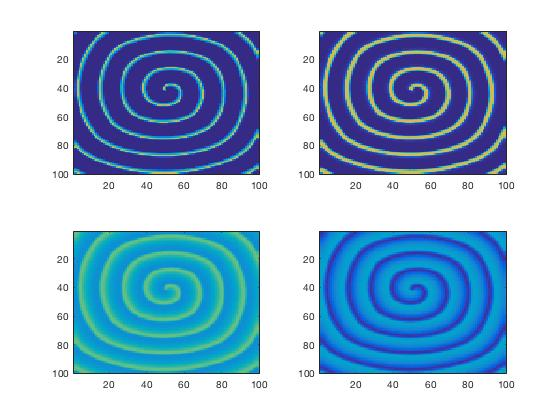
\includegraphics[scale=0.68]{xin_1.jpg}
\caption{$V,m,n,h$函数的螺旋波图样}
% \label{图}
\end{figure}

\begin{figure}[!ht]
\centering
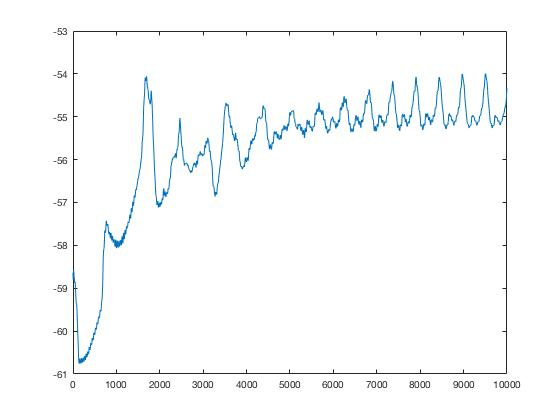
\includegraphics[scale=0.68]{xin_2.jpg}
\caption{$V$的取值变化}
% \label{fig:label}
\end{figure}


\section{HH模型输入为Gamma噪声的相干共振}

我们考虑
\begin{align}
\notag C_m \d V_{ij} &= -\left[\gk (n_{ij})(V_{ij} - \vk) + \gna(m_{ij},h_{ij})(V_{ij}-\vna) + \gl (V_{ij}- \vl) \right] \ud t\\
&+ \d I_{syn}(t) +D(V_{i-1j}+V_{i+1j}+V_{ij-1}+V_{ij+1}-4V_{ij}) \ud t\\
\d y_{ij} &= \left[\alpha (V_{ij})(1-y_{ij})-\beta (V_{ij})y_{ij}\right] \ud t, \quad y=m,h,n
\end{align}
其中,突触输入$I_{syn}(t)$是一系列更新过程的求和,根据Feng\cite{feng2006dynamics}的推导,$\d I_{syn}(t)$可以写成以下形式:
\begin{align}
\d I_{syn}(t) = \frac{ap(1-r)}{\lambda} \ud t + \frac{a \alpha}{\lambda^{\frac{3}{2}}} \left[\sqrt{p(1+r^2)} \ud B_t - c_r \ud \xi^{p,r}(t) \right]
\end{align}
其中,$B_t$是一个标准布朗运动,$r$是静息输入和兴奋输入之比,$\xi^{p,r}$是一个满足以下式子的Ornstein–Uhlenbeck过程:
\begin{align}
\d \xi^{p,r}(t) &= - \xi^{p,r}(t) \ud t + \sqrt{p(1+r^2)} \ud B_t \\
\notag \xi^{p,r}(0) & =0
\end{align}
我们进一步假设$T$是一个遵循Gamma分布的变量,且其对应的密度函数为
\begin{align}
f(t)=\left(\dfrac{1}{\mu}\right)^{\kappa} \dfrac{t^{\kappa-1}e^{-t/mu}}{\tau(\kappa)}
\end{align}
经过Feng\cite{feng2006dynamics}的推导,我们有
\begin{align}
\lambda &= \kappa \mu \\
\alpha ^2 &= \kappa \mu^2 \\
\lambda _3 &= 2 \kappa \mu^3 \\
c_r &= 2 - \sqrt{4+\frac{\lambda^3}{3\alpha^2}+\frac{\alpha^2}{\lambda}-\frac{2\lambda_3}{3\alpha^2}}
\end{align}
经此,我们得到Hodgkin-Huxley神经元晶格模型Gamma突触输入诱导时空斑图的模型如下:
\begin{align}
\notag C_m \ud V_{ij} &= -\left[\gk (n_{ij})(V_{ij} - \vk) + \gna(m_{ij},h_{ij})(V_{ij}-\vna) + \gl (V_{ij}- \vl) \right] \ud t \\
\notag & + \dfrac{ap(1-r)}{\kappa \mu} \ud t
+ \dfrac{a}{\sqrt{\kappa^2 \mu}} \left[ \sqrt{p(1+r^2)} \ud B_t -  \left(2-\sqrt{4+ \dfrac{\kappa^2 \mu}{3}-\dfrac{\mu}{3}} \right) 
\d \xi ^{p, r} _t \right]\\
%\right.\\ 
& %\left. \times \left(-\xi^{p,r}(t) + \sqrt{p(1+r^2)} \d B_t \right) \right] 
+ D(V_{i-1j}+V_{i+1j}+V_{ij-1}+V_{ij+1}-4V_{ij}) \ud t
\end{align}

其中,
\begin{align*}
&V_0 = V_{rest} = B_0\\
&\xi^{p,r}(0) = 0\\
&\kappa > {0, 1-12/ \mu}
\end{align*}

在程序实现中,我们取$a=0.5\mv, b=ar, p=10$,并不断改变$r$的取值得到以下情况的斑图情况,可以发现,在足够长的步数下,当$r$不够大时,模型均可趋向于稳定的螺旋波图样。当$r$取的较大时(例如$r=5$时),模型将不再生成螺旋波图样。

\clearpage

\begin{figure}[!ht]
\begin{minipage}[!ht]{0.5\linewidth}
\centering
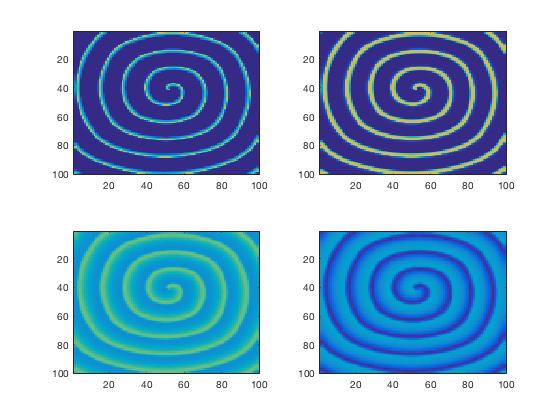
\includegraphics[width=3.0in]{p10r0_1.jpg}
\caption{$r=0$,即所有输入信号均为兴奋}
% \label{fig:side:a}
\end{minipage}%
\begin{minipage}[!ht]{0.5\linewidth}
\centering
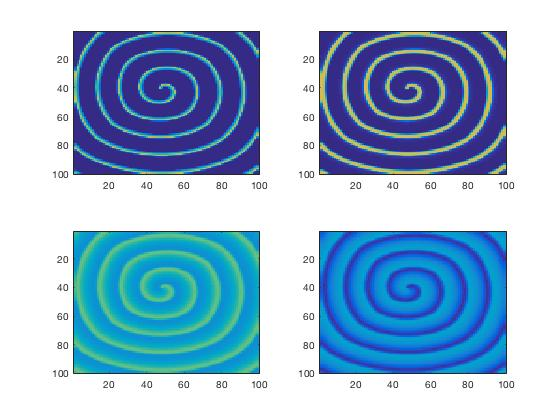
\includegraphics[width=3.0in]{p10r0_2_1.jpg}
\caption{$r=0.2$}
% \label{fig:side:b}
\end{minipage}
\end{figure}

\begin{figure}[!ht]
\begin{minipage}[!ht]{0.5\linewidth}
\centering
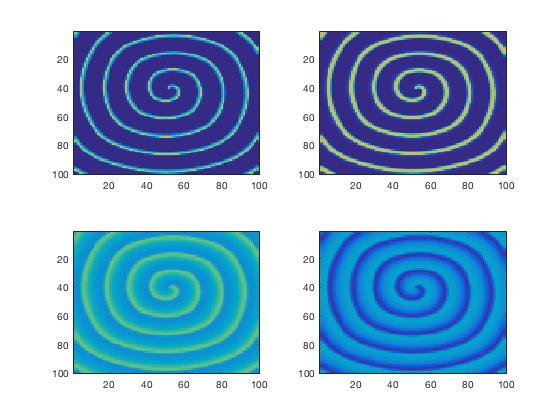
\includegraphics[width=3.0in]{p10r0_5_1.jpg}
\caption{$r=0.5$}
% \label{fig:side:a}
\end{minipage}%
\begin{minipage}[!ht]{0.5\linewidth}
\centering
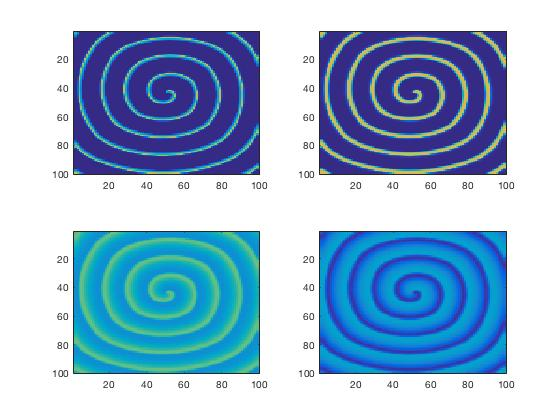
\includegraphics[width=3.0in]{p10r0_8_1.jpg}
\caption{$r=0.8$}
% \label{fig:side:b}
\end{minipage}
\end{figure}

\begin{figure}[!ht]
\begin{minipage}[!ht]{0.5\linewidth}
\centering
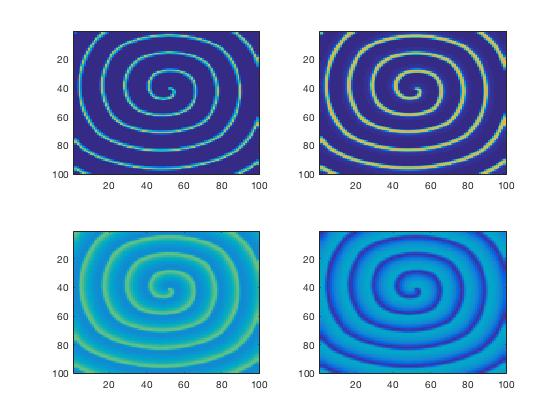
\includegraphics[width=3.0in]{p10r1_1.jpg}
\caption{$r=1$}
% \label{fig:side:a}
\end{minipage}%
\begin{minipage}[!ht]{0.5\linewidth}
\centering
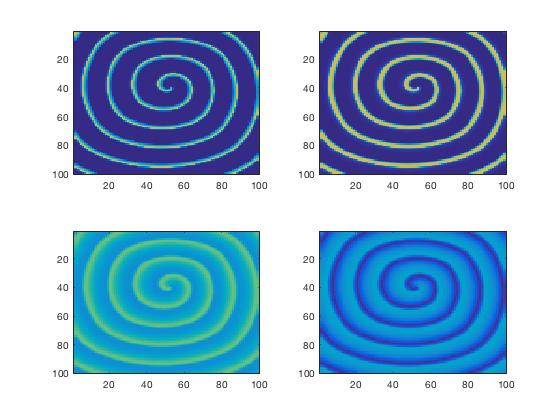
\includegraphics[width=3.0in]{p10r2_1.jpg}
\caption{$r=2$}
% \label{fig:side:b}
\end{minipage}
\end{figure}





\begin{figure}[!ht]
\begin{minipage}[!ht]{0.5\linewidth}
\centering
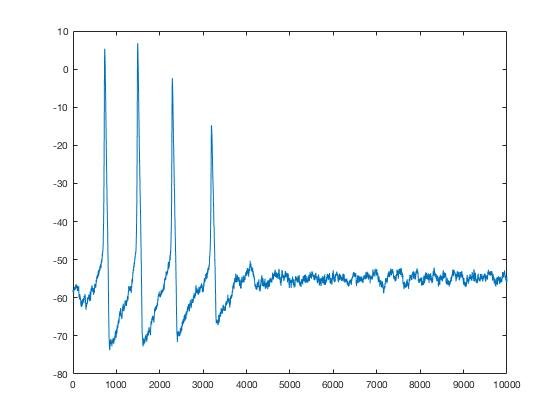
\includegraphics[width=3.0in]{p10r0_2.jpg}
\caption{$r=0$,即所有输入信号均为兴奋}
% \label{fig:side:a}
\end{minipage}%
\begin{minipage}[!ht]{0.5\linewidth}
\centering
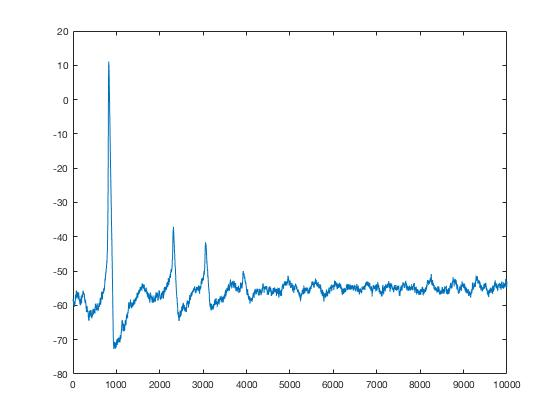
\includegraphics[width=3.0in]{p10r0_2_2.jpg}
\caption{$r=0.2$}
% \label{fig:side:b}
\end{minipage}
\end{figure}


\begin{figure}[!ht]
\begin{minipage}[!ht]{0.5\linewidth}
\centering
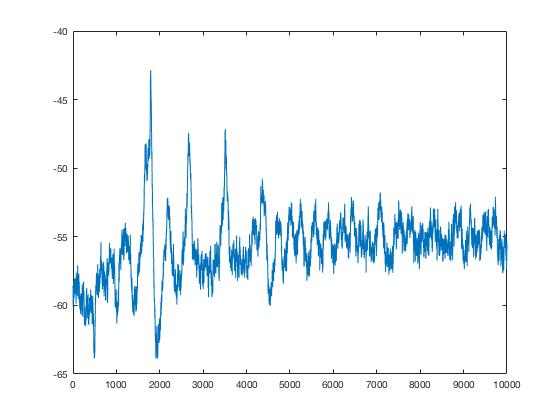
\includegraphics[width=3.0in]{p10r0_5_2.jpg}
\caption{$r=0.5$}
% \label{fig:side:a}
\end{minipage}%
\begin{minipage}[!ht]{0.5\linewidth}
\centering
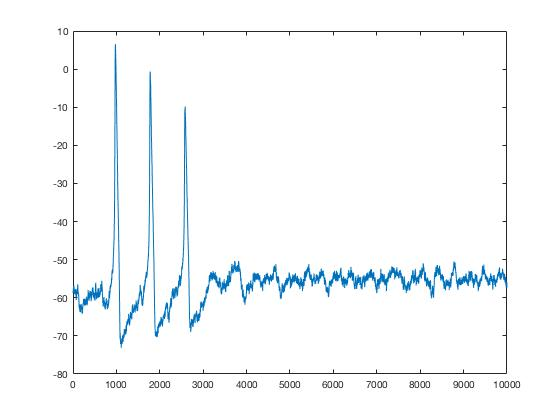
\includegraphics[width=3.0in]{p10r0_8_2.jpg}
\caption{$r=0.8$}
% \label{fig:side:b}
\end{minipage}
\end{figure}

\begin{figure}[!ht]
\begin{minipage}[!ht]{0.5\linewidth}
\centering
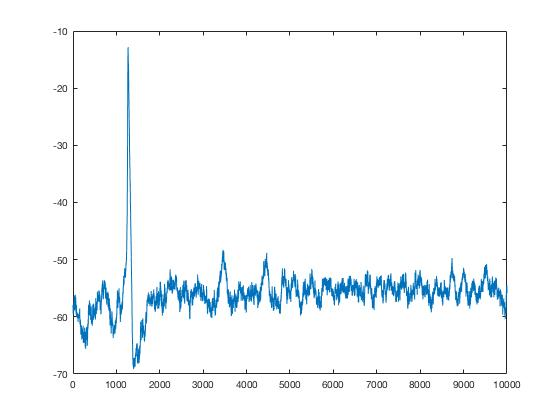
\includegraphics[width=3.0in]{p10r1_2.jpg}
\caption{$r=1$}
% \label{fig:side:a}
\end{minipage}%
\begin{minipage}[!ht]{0.5\linewidth}
\centering
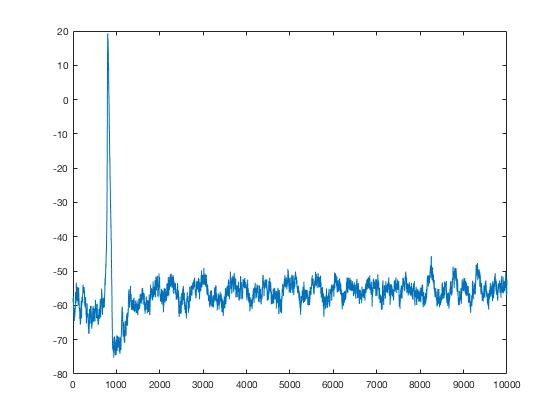
\includegraphics[width=3.0in]{p10r2_2.jpg}
\caption{$r=2$}
% \label{fig:side:b}
\end{minipage}
\end{figure}

\xjtuendcontent


% 将你要引用的文献的 BibTeX 放入 bibliography.bib
\xjtubib{bibliography}

\xjtuappendix

\xjtuappendixchapter{外文原文}
\begin{center}
\noindent
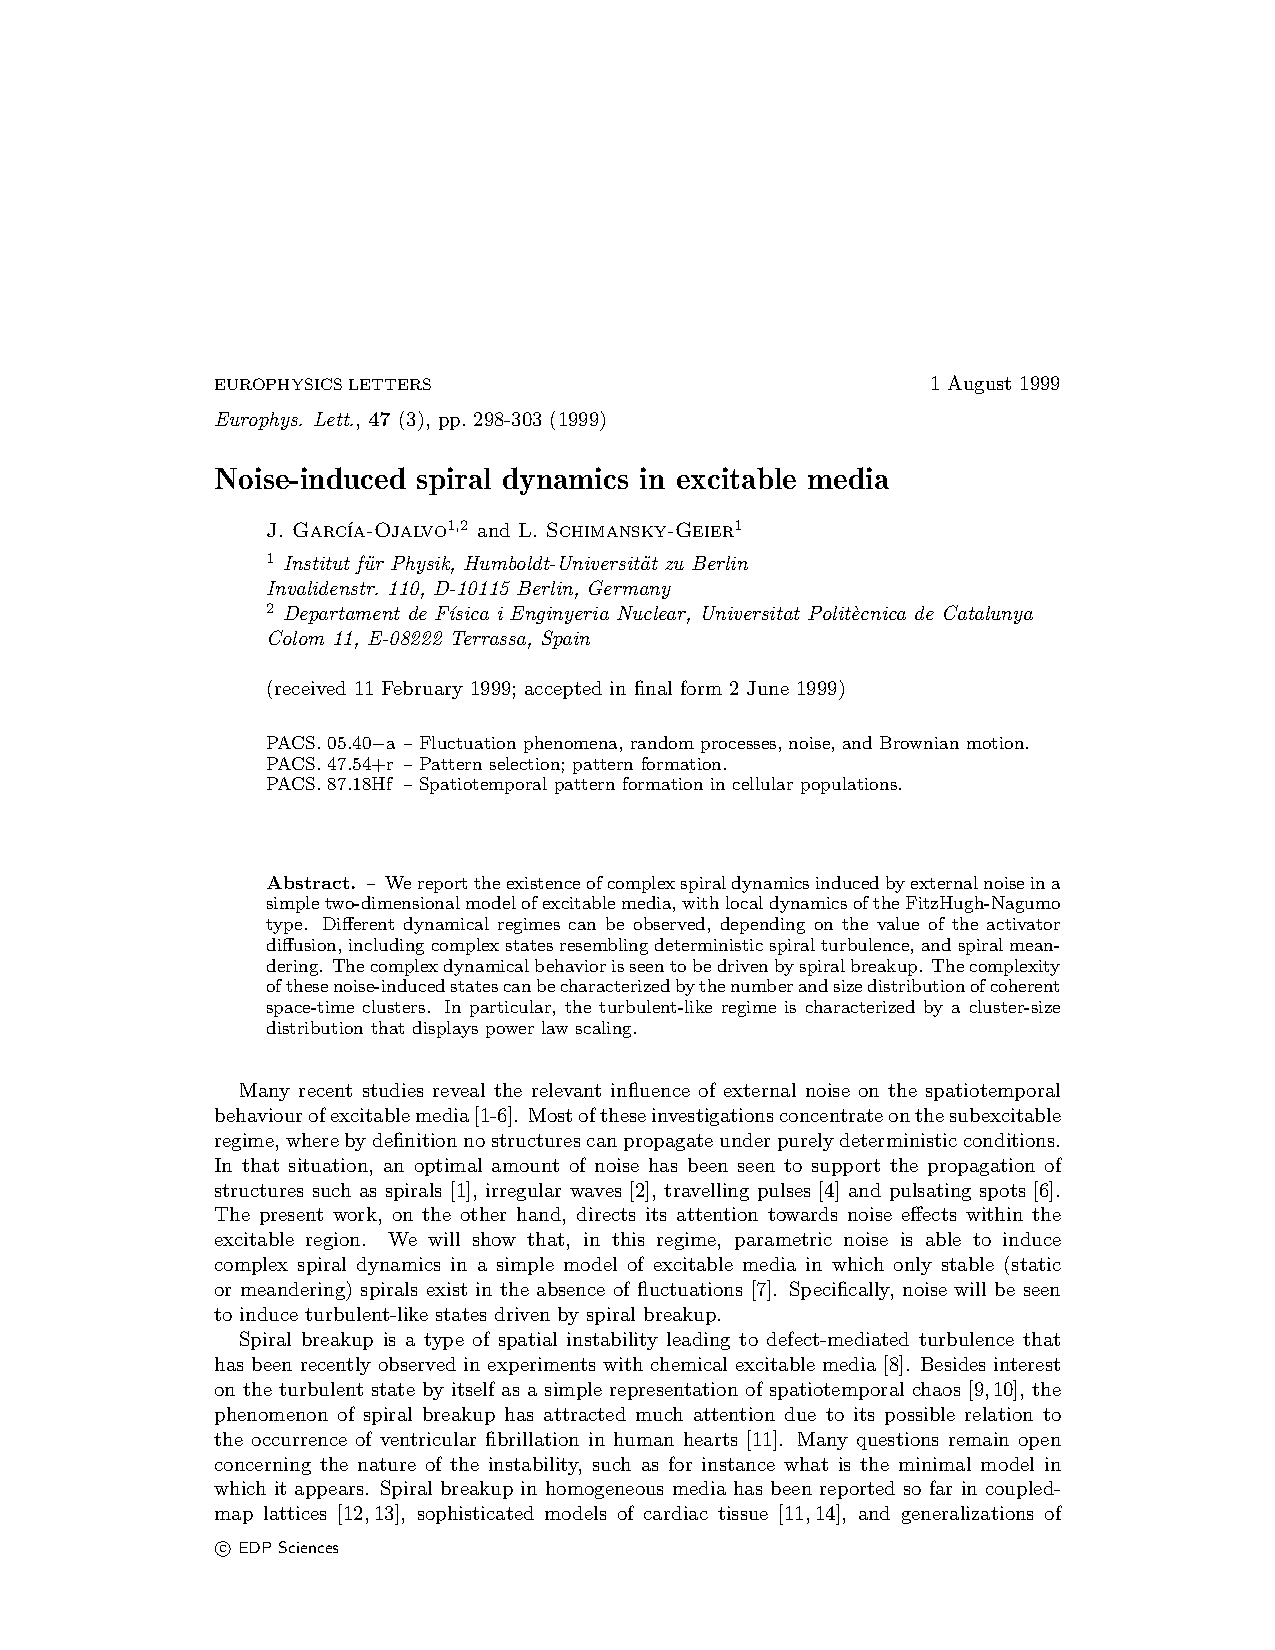
\includegraphics[scale=1]{extra/translation/1}\\
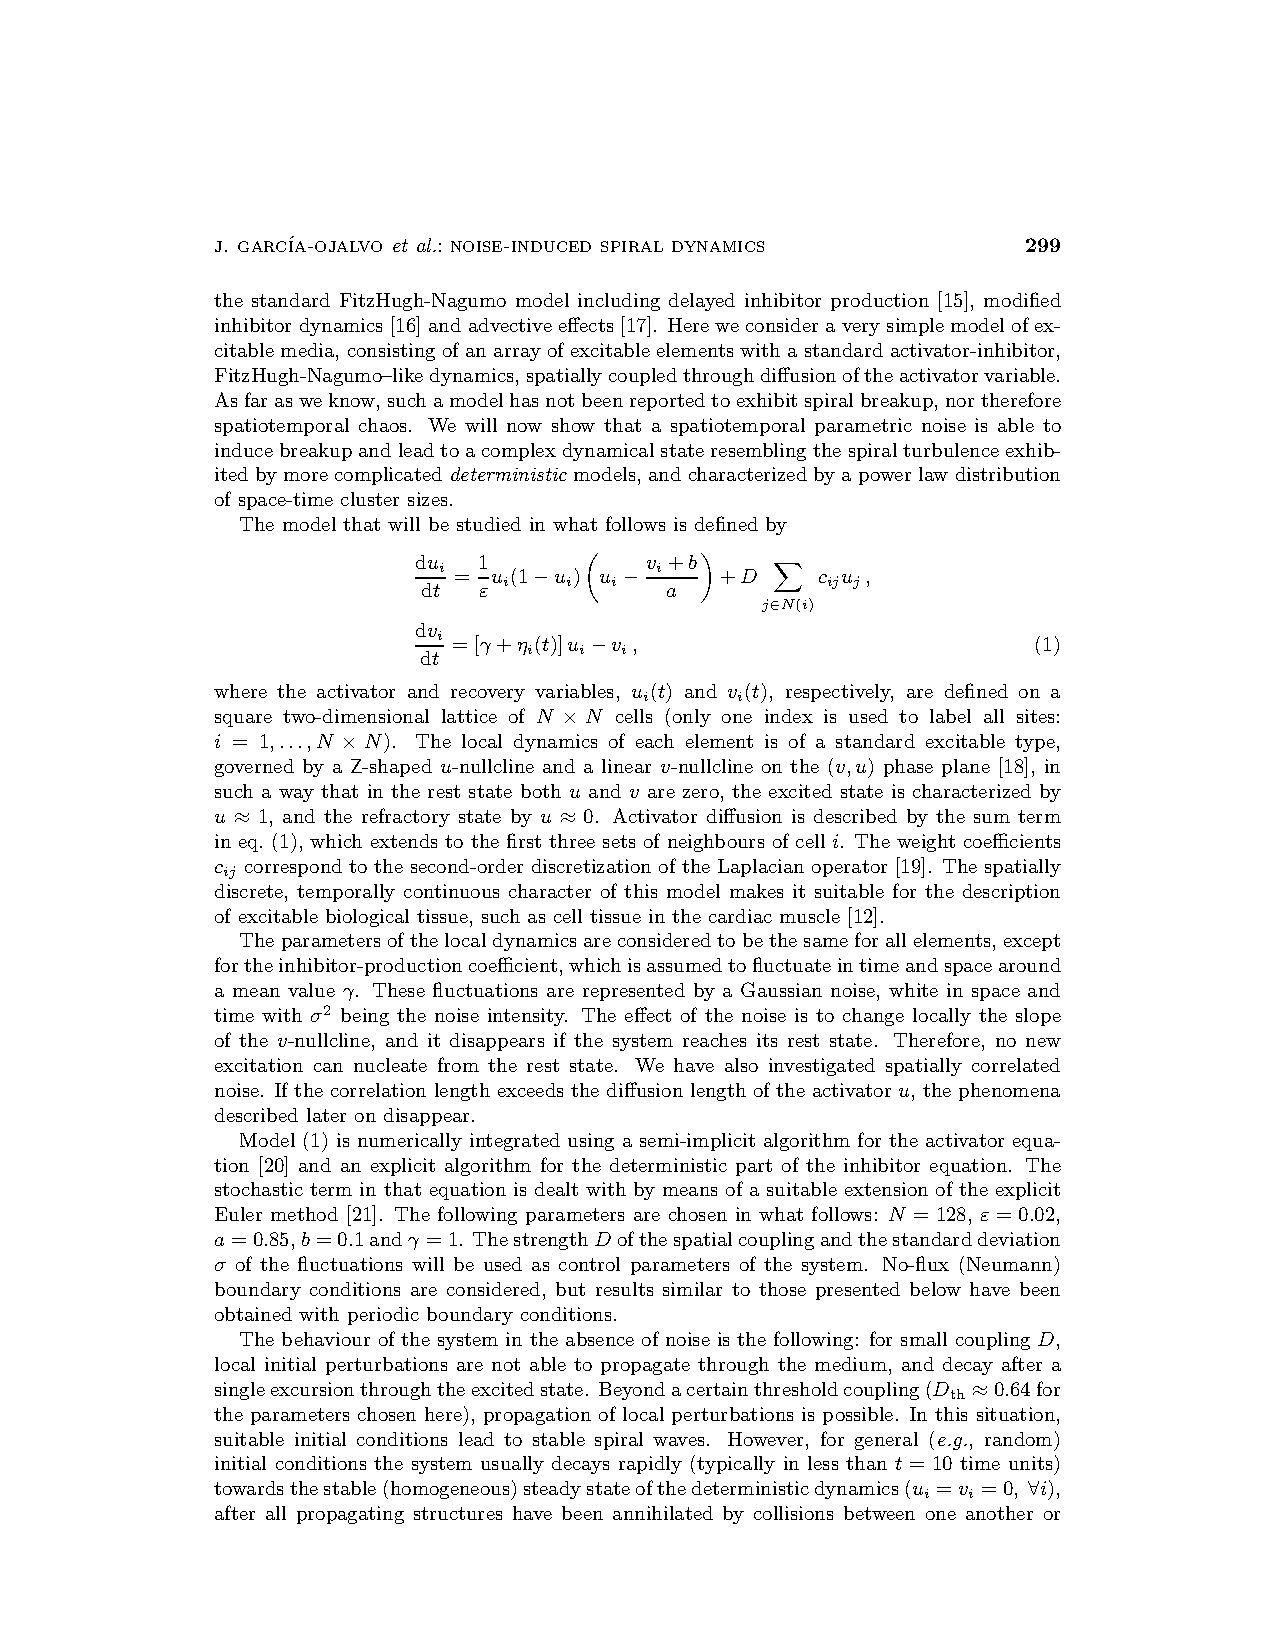
\includegraphics[scale=1]{extra/translation/2}\\
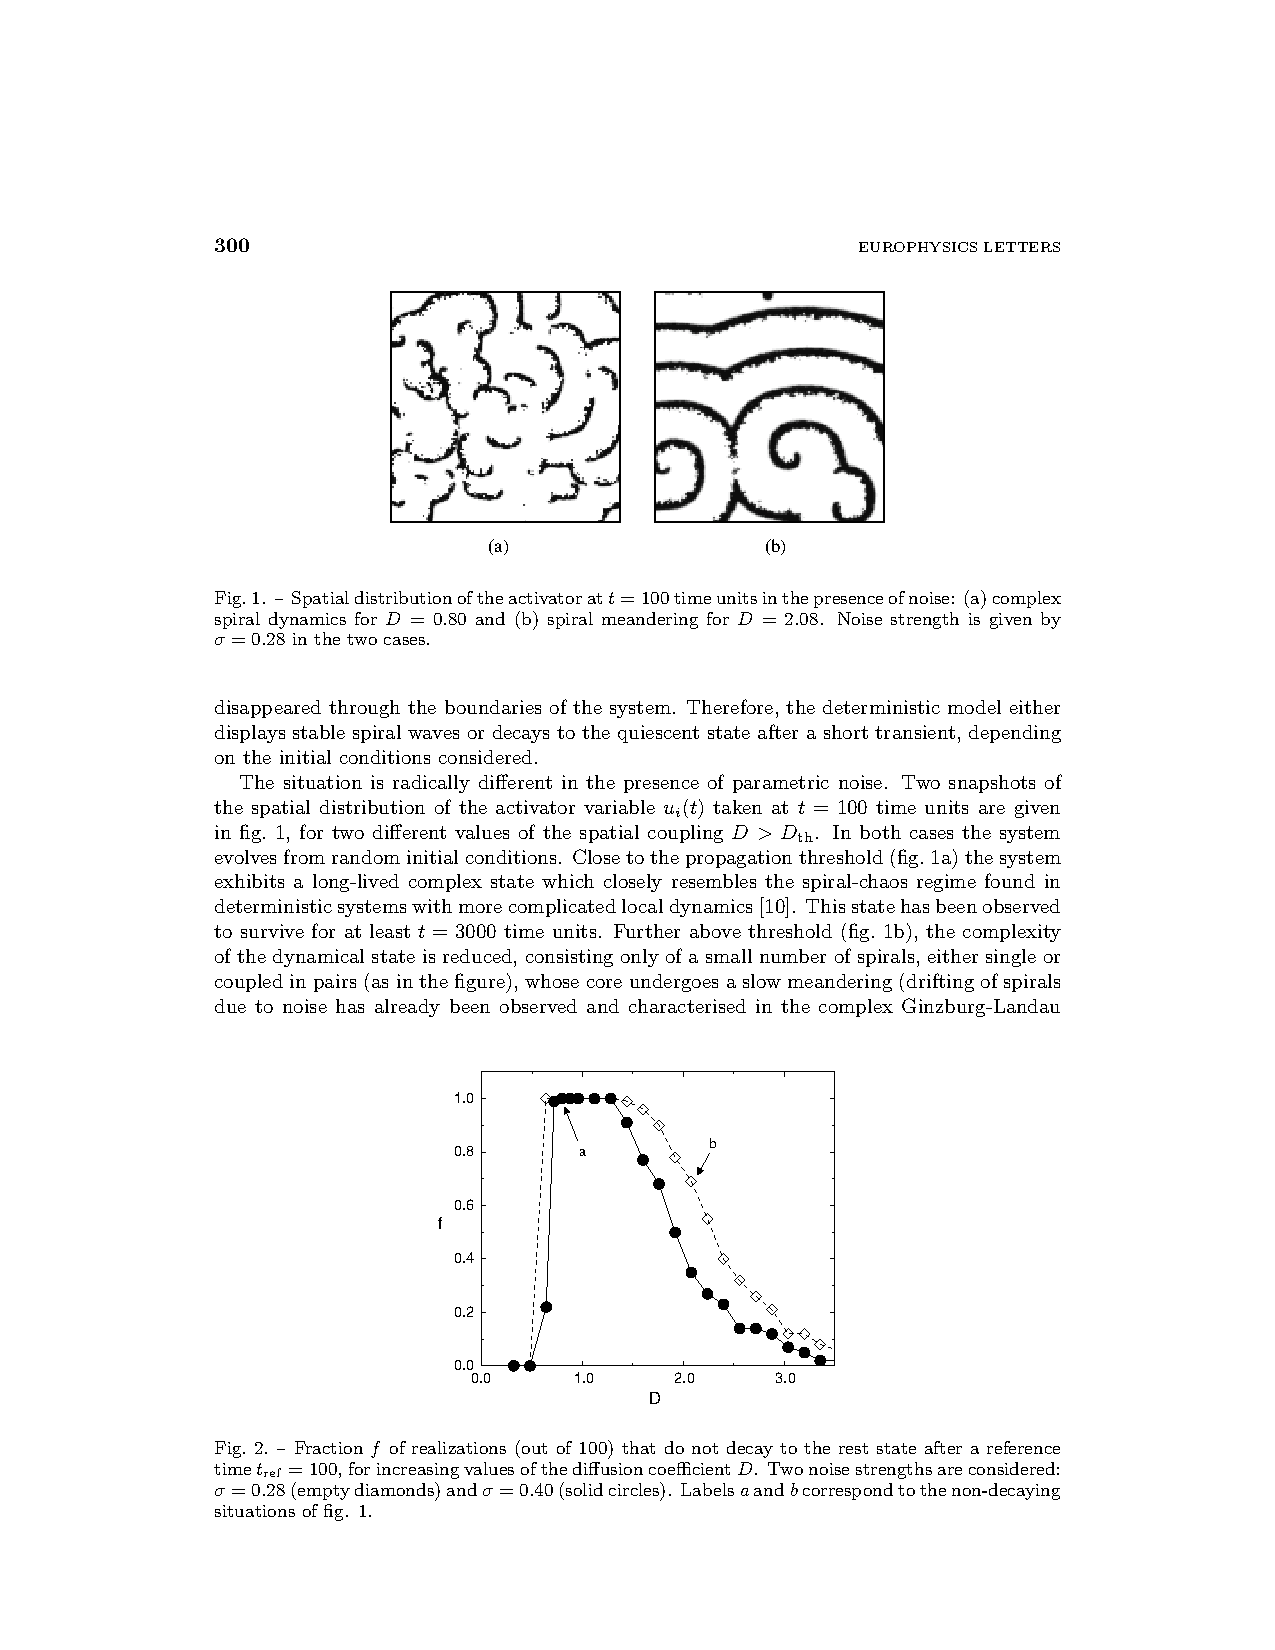
\includegraphics[scale=1]{extra/translation/3}\\
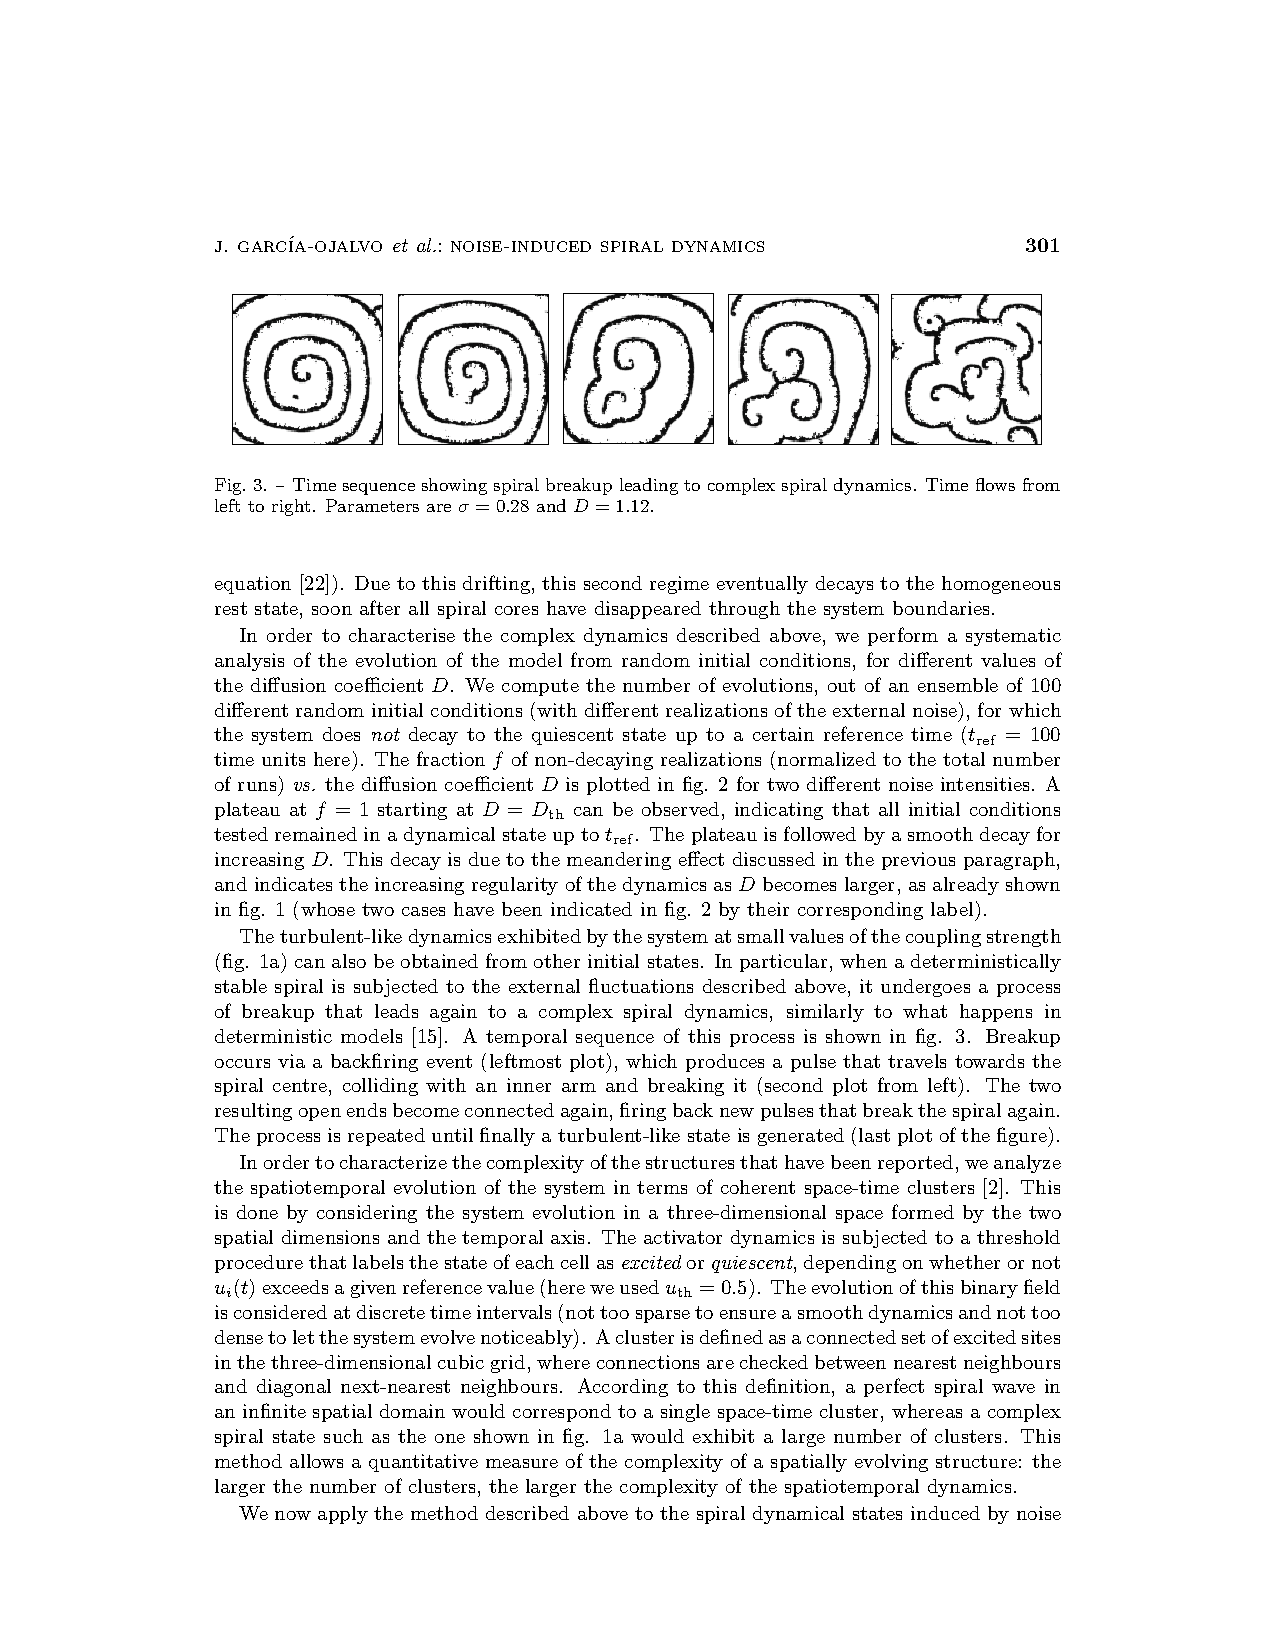
\includegraphics[scale=1]{extra/translation/4}\\
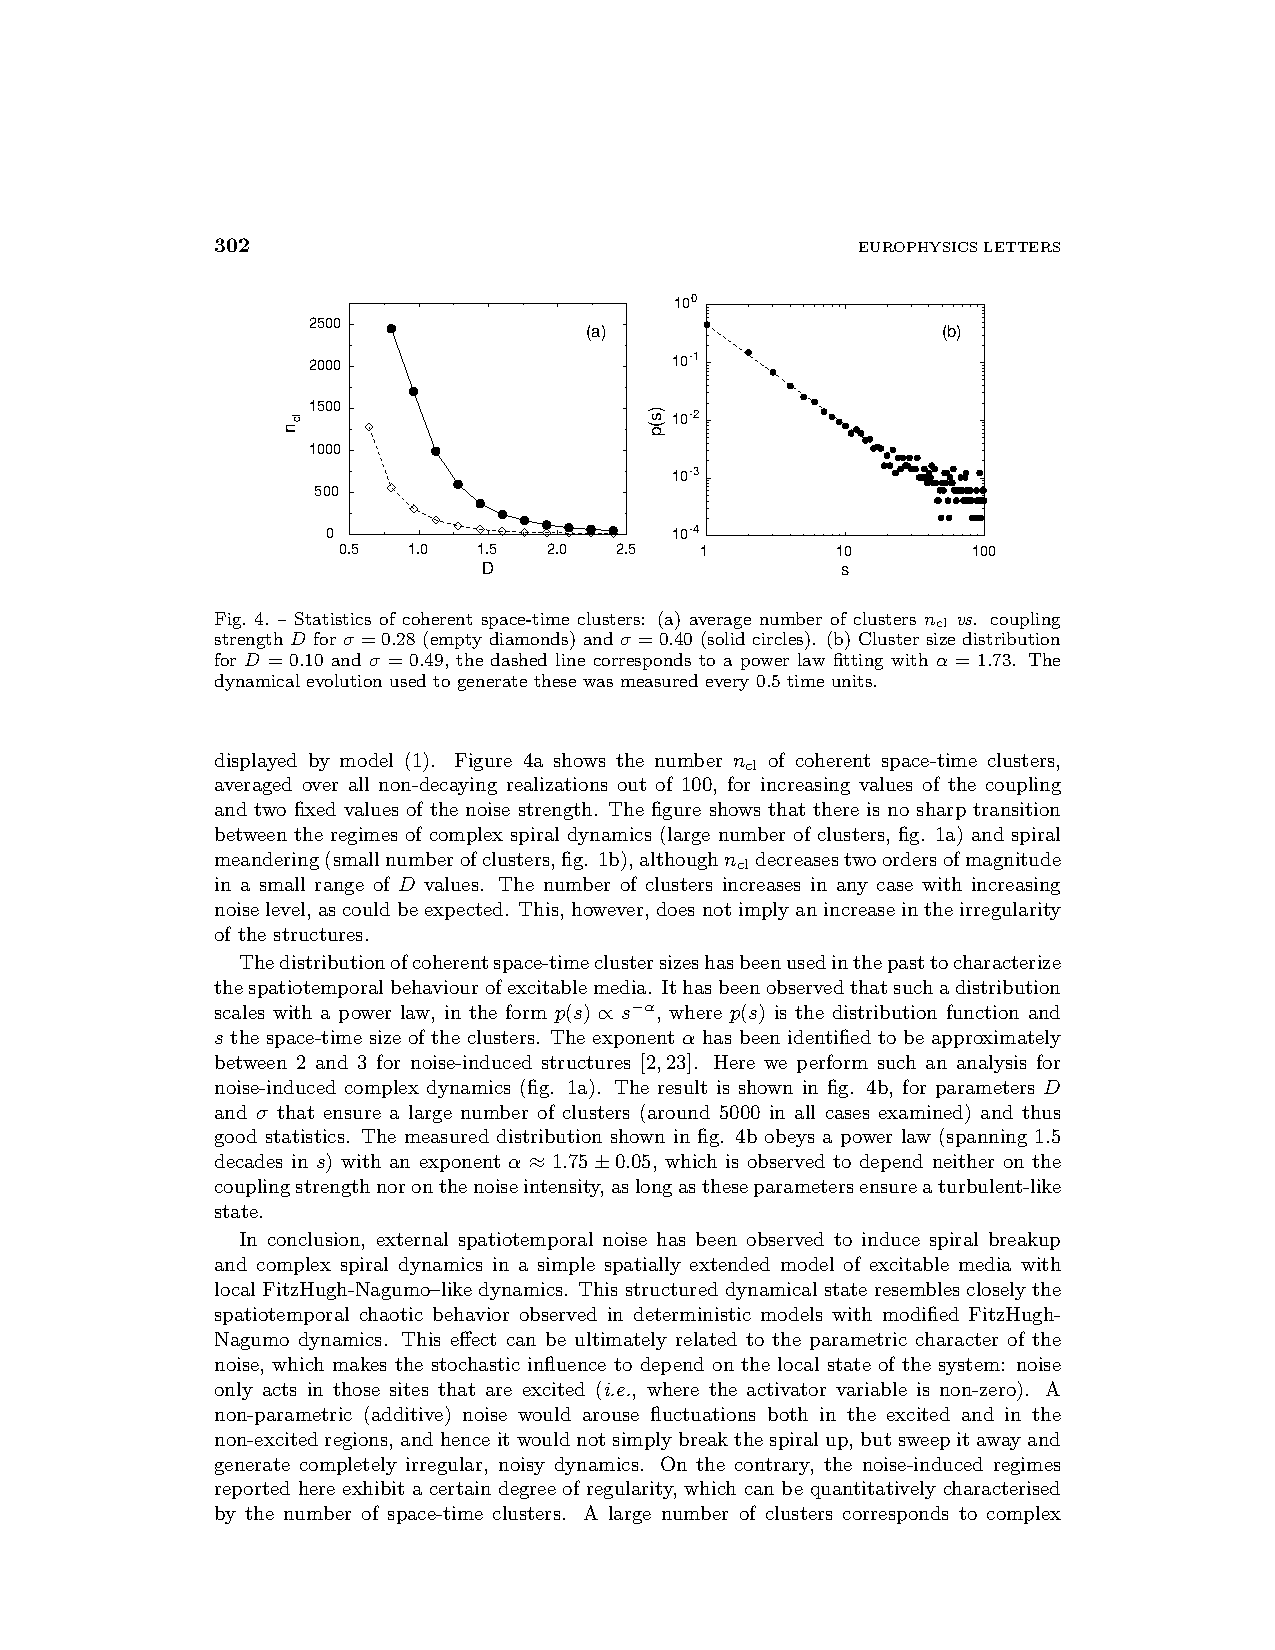
\includegraphics[scale=1]{extra/translation/5}\\
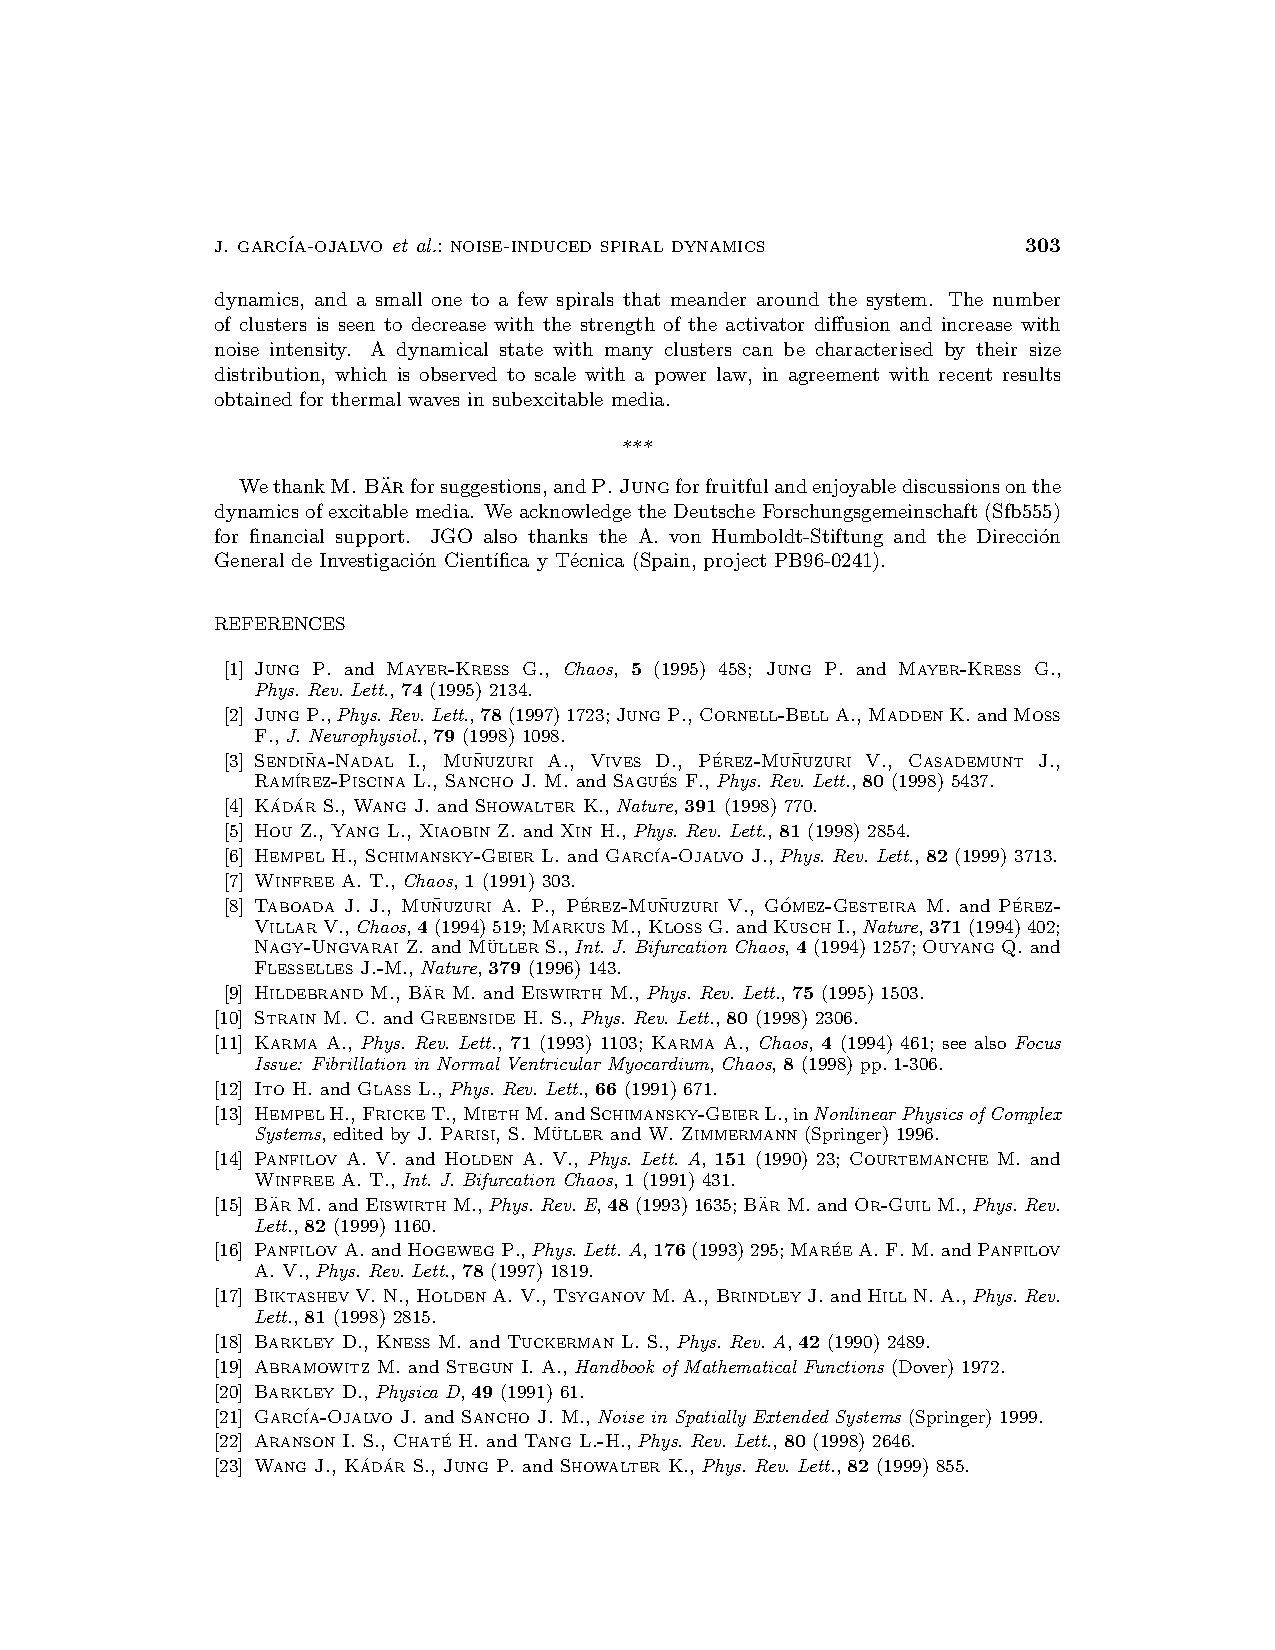
\includegraphics[scale=1]{extra/translation/6}\\
\end{center}

\xjtuappendixchapter{外文翻译: 可激励介质中噪声诱导的螺旋动⼒学}
% 超过一个 section 时用 Appendices, 否则用 Appendix

\newcommand{\apcite}[1]{\textsuperscript{[#1]}}

\xjtuappendixsection{概要}

我们讨论了可激励介质中⼆维模型中由外部噪声引起的复杂螺旋动⼒学的存在性,以及FitzHugh-Nagumo的局部分析。根据激活项的不同取值,可以观察到不同的动⼒学机制,包括类似于确定性螺旋湍流的复杂状态,以及螺旋流。 这种复杂的动态⾏为被认为是由螺旋分裂驱动的。 
特别地,这些噪声引起的状态可以⽤相⼲时空簇的数量和尺⼨分布来表示。 

\xjtuappendixsection{正文}

最近许多研究揭⽰了外部噪声对可激励介质中螺旋动⼒学的影响\apcite{1-6}。 这些研究⼤部分都集中在次优激励上的机制,即根据定义不能在确定性条件下传播的机制。在这种情况下,已经发现了最优的噪声量来⽀持传播
结构如螺旋波\apcite{1},不规则波\apcite{2},⾏进脉冲\apcite{4}和脉动点\apcite{6}。
另⼀⽅⾯,⽬前的研究⼯作将注意⼒转向兴奋部分的噪声效应
。 我们将证明,在这种情况下,噪声是可以在⼀个简单的激励介质模型中诱发
复杂的螺旋动⼒学,其中只有在没有波动的情况下存在稳定的(静态
或流动的)螺旋波\apcite{7}。 具体来说,会看到噪声
诱发的由螺旋分裂驱动的类湍流状态。

\medskip

螺旋分裂是⼀种由于空间不稳定导致的缺陷介导紊流
最近在⽤化学激发介质进⾏的实验中可以观察到\apcite{8}。 除了
在湍流状态本⾝作为时空混沌的简单表⽰\apcite{9,10}
螺旋分裂现象由于其与⼼室颤动可能存在的关系⽽受到了很多关注
\apcite{11}。 关于不稳定性的性质仍然存在许多问题
,例如最⼩模型在哪里出现
。 迄今为⽌,已经发现出现在同质介质中的耦合映象格子\apcite{12,13},⼼脏组织复杂的模型\apcite{11,14},和包括延迟抑制项的标准FitzHugh-Nagumo模型\apcite{15}中的螺旋破裂进⾏了
抑制剂动⼒学\apcite{16}和平流效应\apcite{17}的修改。 在这⾥我们考虑⼀个⾮常简单的可激励机制,是一个由⼀系列含有标准激活项-抑制项的可激发元素组成的FitzHugh-Nagumo类动⼒系统。它通过激活变量的扩散项在空间上耦合。
据我们所知,还没有相关文献讨论这样⼀个模型的螺旋分裂和
时空混沌现象。 现在我们将证明⼀个时空参数噪声能够
诱发噪声分裂并
用一个更复杂的确定性模型表示的类似螺旋湍流展现的复杂动⼒学状态,并以幂律分布的时空簇类为特征。
\medskip
我们将研究一下模型:
\begin{align}
\dfrac{du_i}{dt}&=\dfrac{1}{\epsilon}u_i(1-u_i)(u_i-\dfrac{v_i+b}{a})+D\sum_{j \in N(i)}c_{ij}u_j\\
\notag \dfrac{dv_i}{dt}&=[\gamma+\eta_i(t)]u_i-v_i
\end{align}
其中激活项和抑制项$u_i(t),v_i(t)$定义在一个$N\times N$的二维晶格上。每项的局部动态由$( v,u )$相平⾯\apcite{18}上的Z形$u$的零斜率线和线性的$v$的零斜率线控制,
在这种⽅式下,在静息状态下, $u$ 和$v$ 都是零,兴奋态的特征在于
$u \approx 1$,去兴奋态时$u \approx 0$。 激活项的扩散由等式(1)的求和表示。 权重系数
$c_{ij}$对应于拉普拉斯算⼦的⼆阶离散化\apcite{19}。 在空间上
这种模型的离散,时间的连续特性使其适⽤于描述
可兴奋的⽣物组织,如⼼肌细胞组织\apcite{12}。

\medskip
在局部动⼒学中参数都被认为是相同的
,除了抑制项对于时间和空间周围是波动的
,其平均值$\gamma$。 这些波动由噪⾳强度为$\sigma^2$⾼斯噪声表⽰。 噪声的主要影响为局部改变$V$的零斜率线的斜率,并在系统达到其静⽌状态的时候消失。 因此,静息状态不能产生没有新的
激发。 我们还调查了空间相关性
噪声。 如果相关长度超过激活项$u$的扩散长度 ,后述讨论的现象
会消失。

\medskip
对于模型(1),激活方程主要⽤半隐式算法来数值积分
\apcite{20},而抑制剂⽅程的确定性部分主要使用显式算法,随机项的计算则主要通过显式
欧拉⽅法\apcite{21}。 参数取值如下: $N = 128,\epsilon = 0.02,a = 0.85,b = 0.1,\gamma = 1$。空间耦合的强度$D$ 和标准偏差
$\sigma$ 将被⽤作系统的控制参数。模型满足Neumann
边界条件,但结果与周期性边界条件得到的结果类似。

\medskip
系统在没有噪声的情况下的动力学行为如下:对于较小的耦合系数$D$ ,
局部初始扰动不能通过介质传播,并在简单的偏移之后衰减。 当$D$超过⼀定阈值($D_{th} \approx 0.64$),局部扰动的传播是可能的。 在这个情况下,
合适的初始条件会导致稳定的螺旋波。 但是,对于⼀般的初值条件,
系统通常会迅速衰减(通常⼩于 $t = 10$个时间单位)
到确定性动⼒学的稳定(均匀)稳定状态( $u_i = v_i = 0,\forall i$ ),这时所有传播行为在边界通过碰撞而消失。 因此,确定性模型可能会
产生稳定的螺旋波或衰减到短暂瞬态后的静⽌状态,取决于系统的
初始条件。

\medskip
在存在噪声的条件下情况会完全不同。图1的两个图
给出当$D> D_{th}$的两个不同取值下在$t = 100$个时间单位下激活变量 $u_i(t)$ 的空间分布。 在这两种情况下的系统
均从随机的初始条件演变⽽来。 在接近传播阈值(图1a)时系统
表现出⼀种长期复杂的状态,与
确定性系统中发现的螺旋混沌现象⾮常相似,且具有更复杂的局部动态\apcite{10}。 这种状态已被观察到
可以⾄少在$ t = 3000$个时间单位中⽣存 。当远超过阈值时(图1b),动⼒状态的复杂性减少,只包括少量的螺旋,⽆论是单个还是成对出现的(如图中所⽰),其内核经历了缓慢的偏移(由于噪声产生的螺旋漂移现象
已经在复杂的Ginzburg-Landau方程中被观察到\apcite{22})。 由于这种漂移,当螺旋波的内核在系统边界消失后,第二种状态很快衰减到静息状态。

\begin{figure}[!ht]
\centering
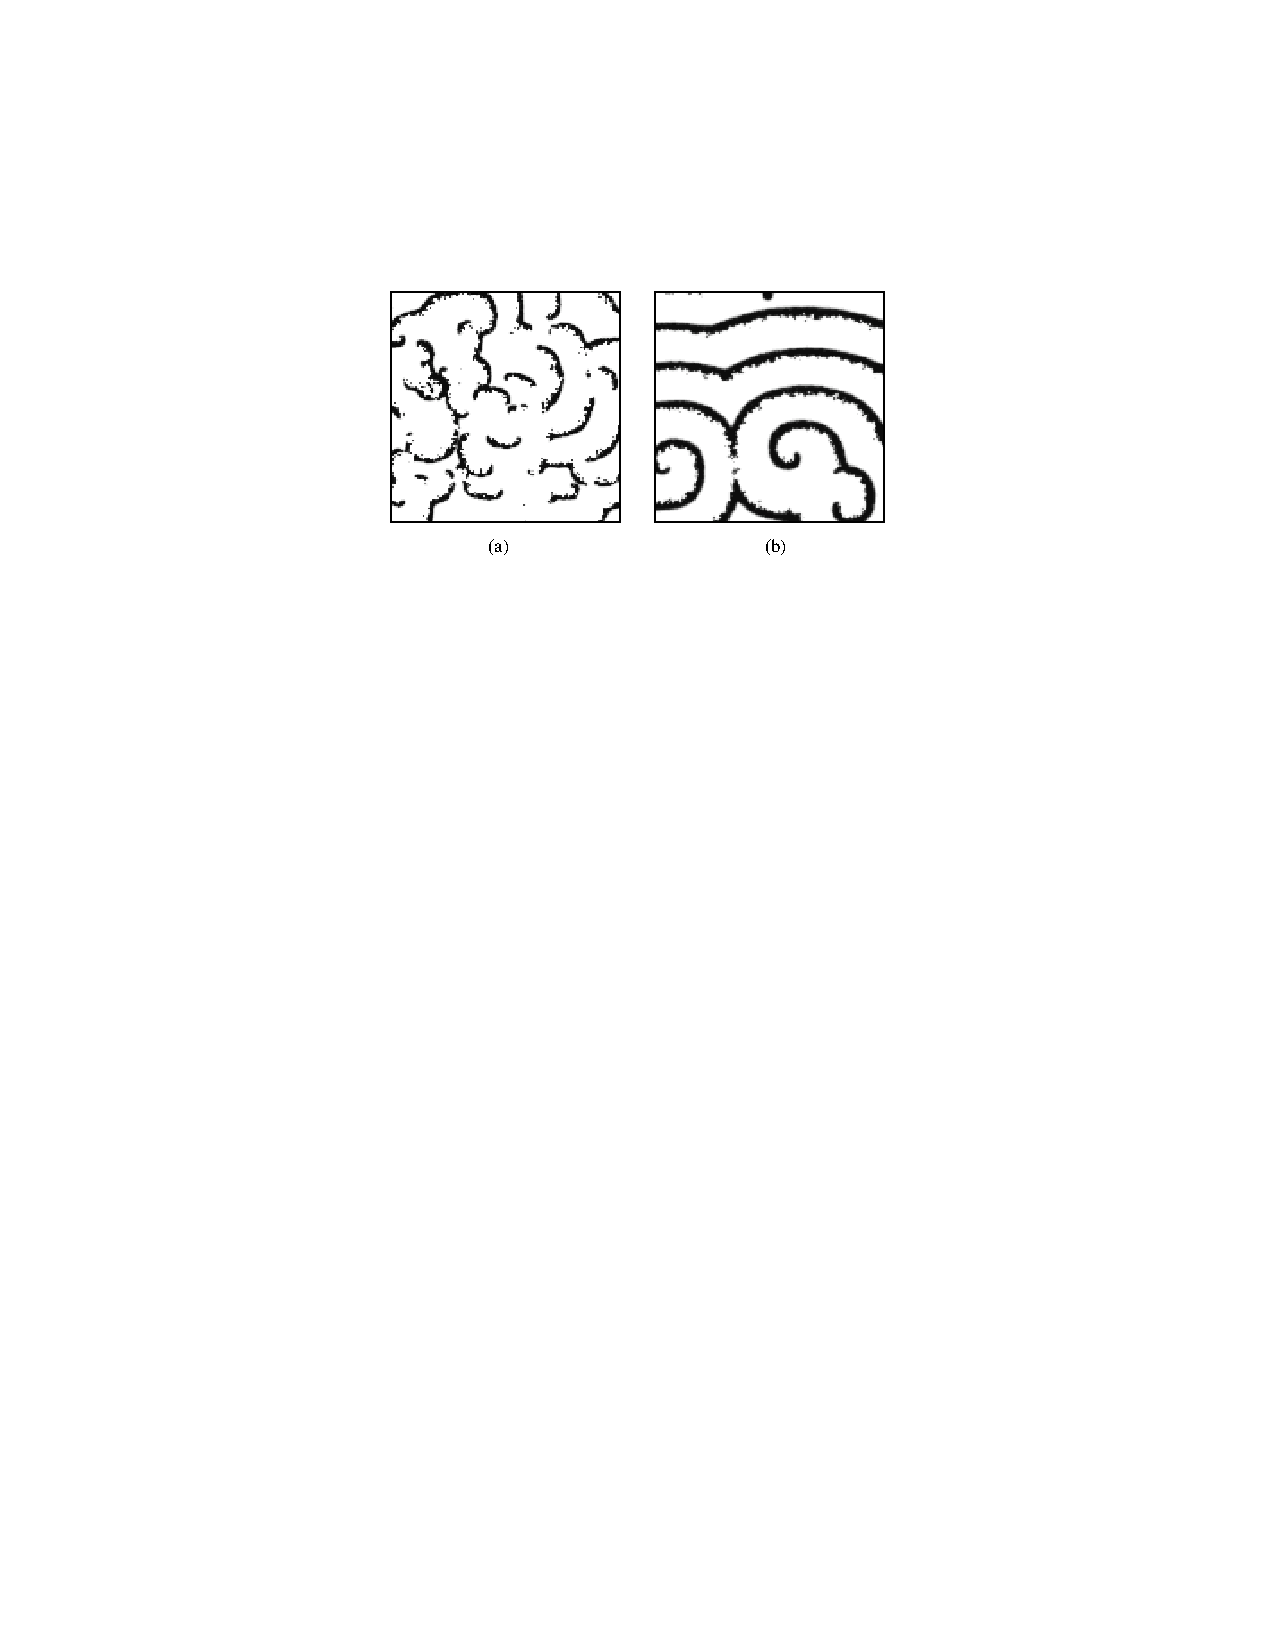
\includegraphics[scale=1]{fig1.pdf}
\caption{噪声诱导下在$t = 100$个时间单位下激活变量 $u_i(t)$ 的空间分布}
% \label{fig:label}
\end{figure}

\medskip
为了描述上述复杂的动态特征,我们针对不同的
扩散系数$D$来系统演示在随机初始条件下模型的进化。 我们计算了100个不同的随机初始条件(具有不同的外部噪声实现)下模型的进化, 其中
系统不会在一定时间内($t_{ref} = 100$
个时间单位)衰减到静⽌状态。 图2展示的是在两种不同的噪声强度下未衰减的实现与总的实现个数的比例$f$与扩散系数$D$的关系。 我们可以观察到从$D = D_{th}$开始$f$先维持在 $f = 1$不变 ,表明在所有的初始条件
下系统在$t=t_{ref}$前都处于激活状态。 之后随着$D$的增加$f$平稳的减小。 这种减小是由于前⼀段讨论的螺旋漂移现象,
如图1中所示,随着$D$变⼤, 系统的动力学行为也更加规律。

\begin{figure}[!ht]
\centering
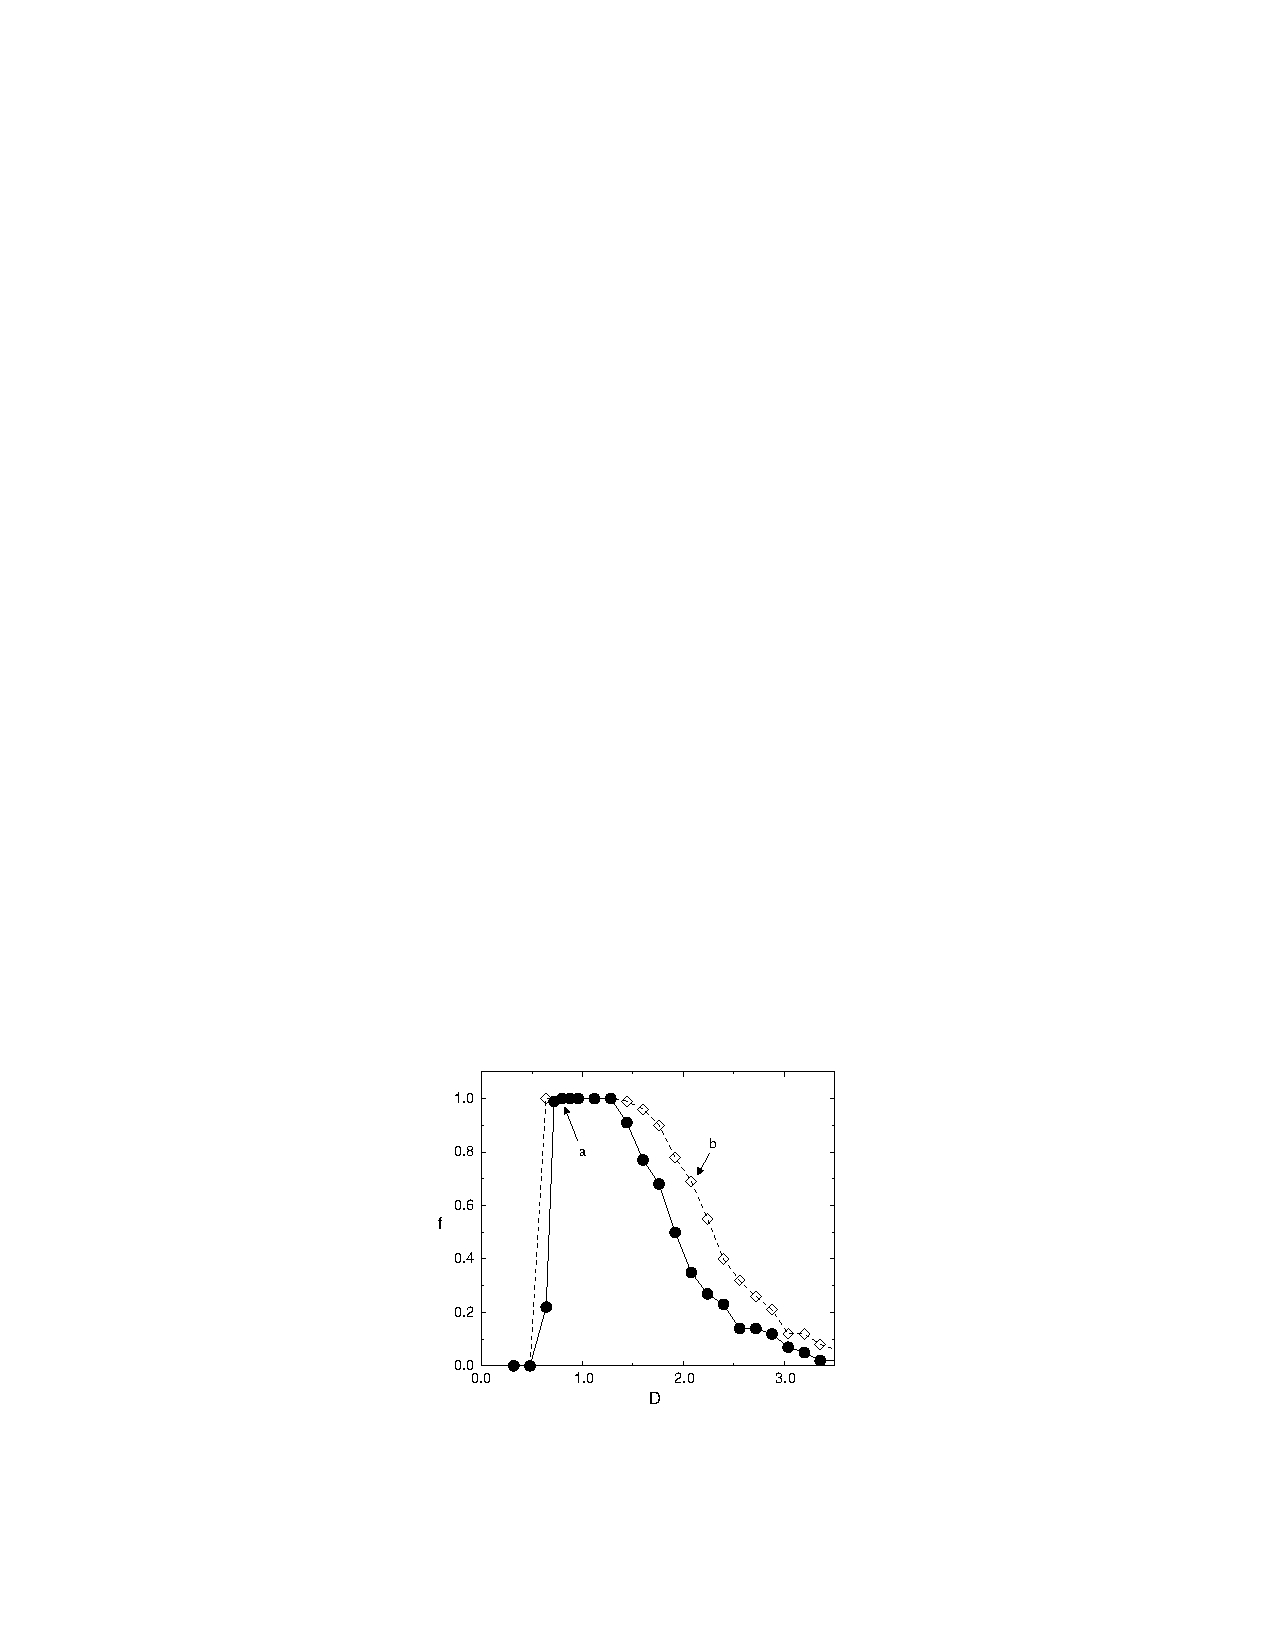
\includegraphics[scale=1]{fig2.pdf}
\caption{两种不同的噪声强度下未衰减的实现与总的实现个数的比例$f$与扩散系数$D$的关系}
% \label{fig:label}
\end{figure}

\medskip
系统在耦合强度值很⼩的情况下表现出的湍流状态
(图1a)也可以从其他初始状态获得。 特别地,当⼀个确定性的
稳定的螺旋受到上述的外部波动,它会产生分裂并转变为一个复杂的螺旋动⼒学行为,与确定性模型的情形类似
\apcite{15}。 这个过程的时间序列如图3所⽰。 分裂
通过一次回⽕事件(最左边的点)发⽣,这会产⽣⼀个向
螺旋中⼼移动的脉冲,与螺旋波内壁碰撞并打破它(左起第⼆个点)。 由此产生的两个打开的断尾再次连接,发射新的脉冲并再次打破螺旋波。
重复该过程直到最终产⽣类似湍流的状态(图中最后⼀个点)。

\begin{figure}[!ht]
\centering
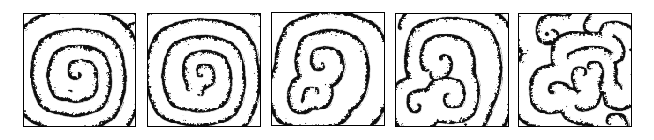
\includegraphics[scale=0.68]{fig3.png}
\caption{螺旋波分裂会产生复杂的螺旋动力学}
% \label{fig:label}
\end{figure}

\medskip
为了描述上述结构的复杂性,我们分析
系统在连续时空集群下的时空演化\apcite{2}。 这个
是通过考虑由两个空间维度和时间轴形成的三维空间中的系统演化来完成的
。 激活态行为主要通过阈值描述
,将每个细胞的状态标记为兴奋或静⽌ ,取决于$u_i(y)$是否
超过一个给定的参考值($u_{th}= 0.5$)。 这两种状态的演变
被认为是在不连续的时间间隔(既不是太稀疏以确保动力行为的光滑性,又不是太密集的让系统很明显的演变)。 ⼀个集群被定义为在三维⽴⽅⽹格中的⼀组兴奋点的连通集,其中路径只连接距离最近或者对角次最近的点。根据定义,在无穷区域上的一个完美的螺旋波对应单个时空集群,而一个如图1a所⽰的复杂的螺旋状态会对应多个时空集群。 这个
⽅法可以定量测量空间演变结构的复杂性:
时空集群的数量越多,时空动态的复杂度就越⼤。

\medskip
我们现在将上述⽅法应⽤于模型(1)中由噪声引起的螺旋波动力行为。 图4a显⽰了连续时空集群的数量 $n_{cl}$ ,
是对超过100次随着耦合值增加和个固定的噪声强度值下的所有⾮衰减实现中取平均的结果。 这个数字表明
在复杂的螺旋动⼒学(多个时空集群,图1a)和螺旋漂移(少量时空集群,图1b)之间没有急剧的转变,尽管$n_{cl}$随着$D$的小幅度减小会降低两个数量级。 在任何情况下集群数量会随着噪声强度增加而增加,然⽽这并不意味着系统变得更加不规律。

\begin{figure}[!ht]
\centering
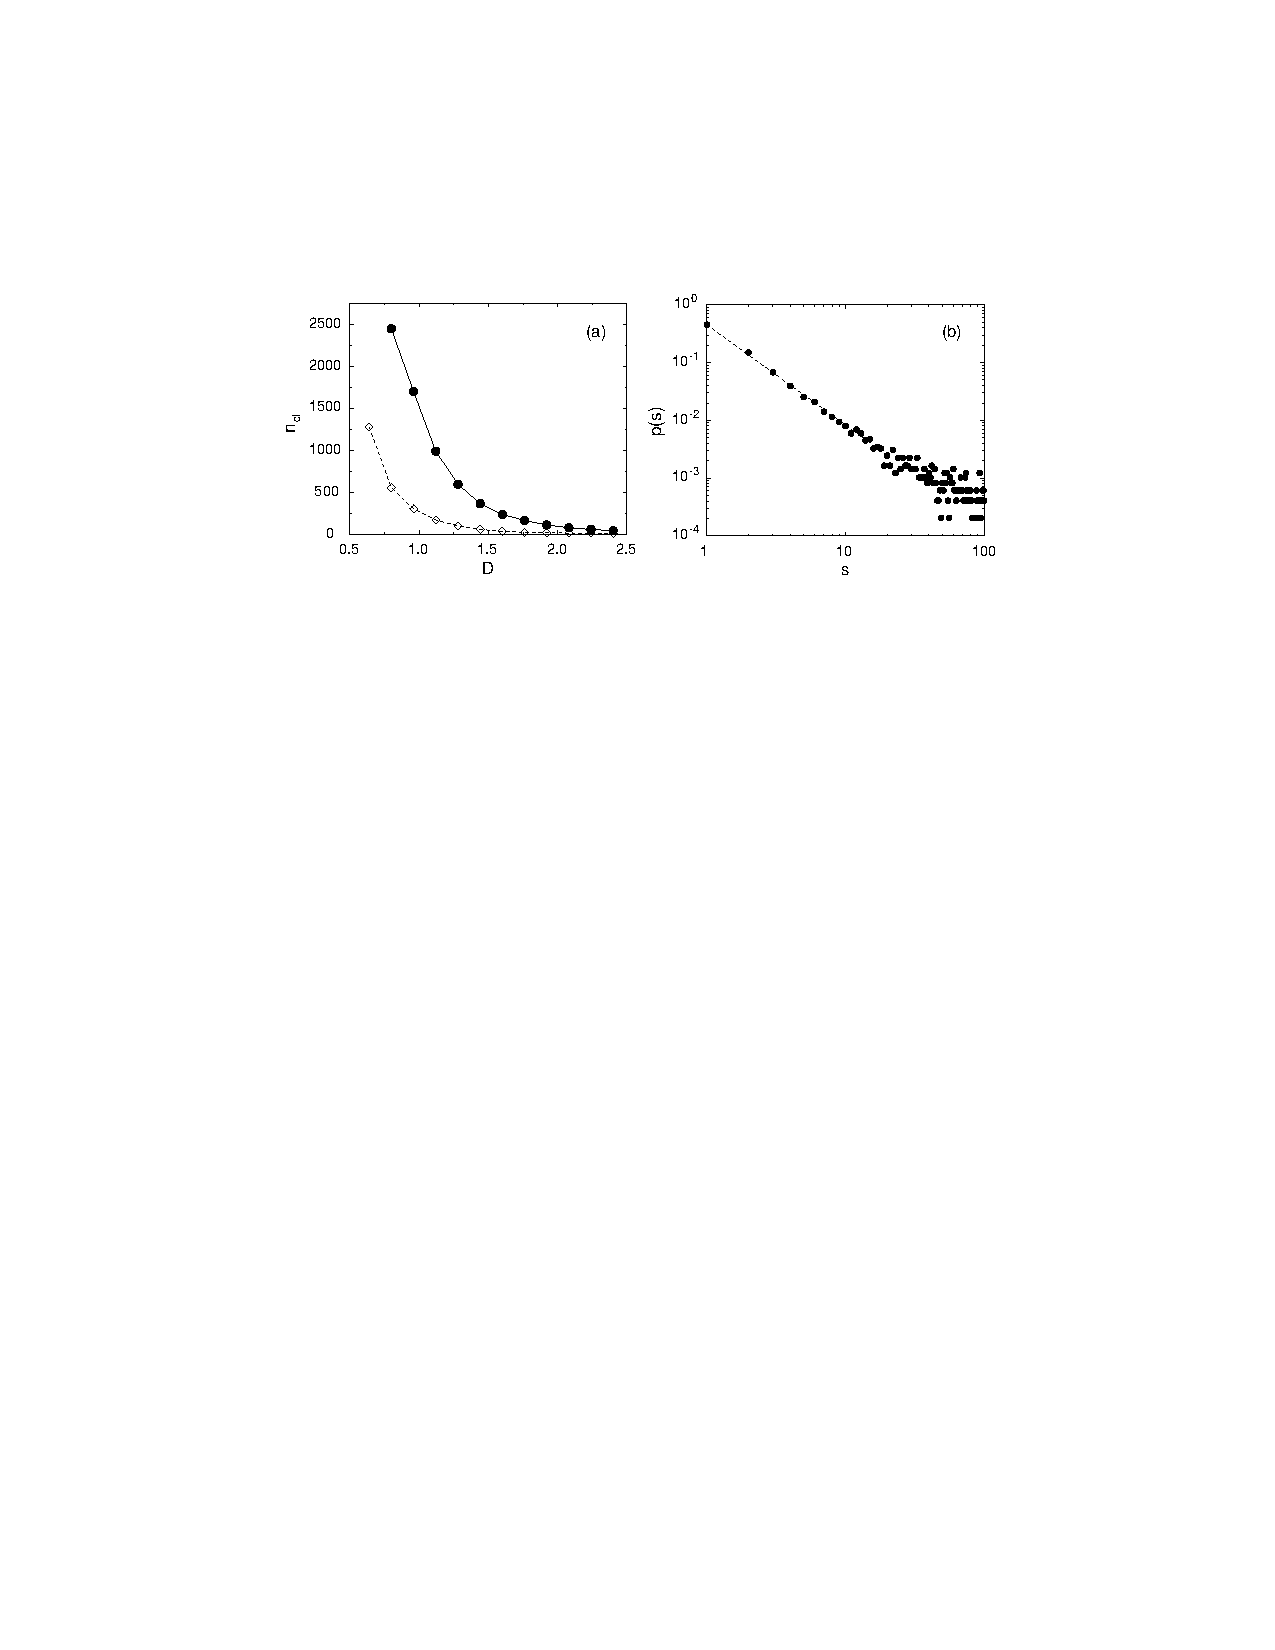
\includegraphics[scale=1]{fig4.pdf}
\caption{连续时空集群的统计性质}
% \label{fig:label}
\end{figure}

\medskip
连续时空集群的分布在过去被⽤来表征
可兴奋介质的时空⾏为。 据观察,这种分布
以幂律定律缩放,形式为$p(s)\propto s^{-\alpha}$,其中 $p(s)$是分布函数,$s$是集群的时空规模。 指数$\alpha$已被确定为近似
在2到3之间的噪声诱导结构\apcite{2,23}。 我们在这⾥对噪声诱导的复杂动⼒学(图1a)进⾏这样的分析。 结果如图4b所⽰,其中参数$D$和$\sigma$保证多个时空集群(在被检验的情况中大概为5000个)的情形。测得的分布遵循幂律定律,其中指数$\alpha \approx 1.75\pm 0.05$,且只要满足在湍流状态下$\alpha$与耦合强度与噪声强度无关。

\medskip
总而言之,外部时空噪声已被观察到可以诱发螺旋破裂
,和在可激励介质中局部FitzHugh-Nagumo类简单的空间扩展模型的复杂的螺旋动⼒行为。 这种结构化的动⼒学状态⾮常类似于
在确定性模型中观察到的时空混沌⾏为。 这种效应最终可能与噪声的特征参数有关
,这使得随机影响取决于系统的局部状态:噪声
仅在那些被激活的点( 即激活变量不为零的地⽅)中起作⽤ 。 ⼀个
另外的⾮参数噪⾳会引起兴奋和
⾮兴奋区域的波动,因此它不会简单地打破螺旋,⽽是产⽣完全不规则的嘈杂的动力学行为。 相反,由噪声引起的机制中
则具有⼀定程度的规律性,并可以被定量地由时空集群的数量来表示
。 多个集群对应于复杂的动态性,少量集群则对应一些螺旋波的漂移现象。 
随着扩散强度和噪⾳强度的增加,集群的数量减少
。 多个集群对应的动力学状态可以⽤它们分布来表征
,其中它们的分布遵循幂律定律,这与最近在次可激励介质中的热波所观察到的结果⼀致。

\bigskip
\begin{center}
***
\end{center}

我们感谢M.Bär的建议,并感谢P. Jung为我们提供了在可激励介质中的动力学行为的富有成果和愉快的讨论。 我们感谢Deutsche Forschungsgemeinschaft(Sfb555)
的财务⽀持。 JGO也感谢A. von Humboldt-Stiftung和Dirección
General de Investigación Cientıfica y Técnica(西班⽛,项⽬PB96-0241)。

\xjtuendappendix

\xjtuspchapter{致谢}{致\qquad 谢}
\iffalse
本文是在西安交通大学的李东升老师与佐治亚理工学院的林治武老师的共同指导下完成的, 受到美国国家科学基金会NSF (grantDMS-1411803)项目的资助. 林治武老师为论文的选题, 文献资料的选择提供了十分有益的指导, 并十分关照本人的工作进展, 使得论文得以顺利完成. 在佐治亚理工学院实习期间, 林治武老师组织的丰富的讨论班与讲座也给予了我很多启发. 同时也需要在此感谢学校拔尖办给予我此次出访机会, 感谢佐治亚理工学院的同僚们的帮助, 让我能够进行这样一项很有意义的科研. 另外, 本毕业设计虽然是在外校完成的, 李东升老师仍然给予了相当细致的关照与充分的支持, 本文的完成离不开他的帮助. 谨向林治武老师与李东升老师致以衷心的感谢! 
\fi

\end{document}
